\documentclass[a4paper,14pt]{extarticle}

% Поддержка русского языка и кодировок
\usepackage[T2A]{fontenc}
\usepackage[utf8]{inputenc}
\usepackage[russian]{babel}

% Настройка полей по ГОСТ
\usepackage{geometry}
\geometry{left=3cm, right=1.5cm, top=2cm, bottom=2cm}

% Разрешение гибких переносов (против вылезания за поля)
\usepackage{hyphenat}
\sloppy
\emergencystretch=3em

% Настройка интервалов и абзацев
\usepackage{setspace}
\onehalfspacing
\usepackage{indentfirst}

% Центрирование всех заголовков разделов и подразделов
\usepackage{titlesec}
\titleformat{\section}
{\normalfont\large\bfseries\centering}{\thesection.}{0.5em}{}
\titleformat{name=\section,numberless}
{\normalfont\large\bfseries\centering}{}{0em}{}
\titleformat{\subsection}
{\normalfont\normalsize\bfseries\centering}{\thesubsection.}{0.5em}{}
\titleformat{name=\subsection,numberless}
{\normalfont\normalsize\bfseries\centering}{}{0em}{}

% Математические пакеты
\usepackage{amsmath, amsfonts, amssymb}

% Графика и таблицы
\usepackage{graphicx}
\usepackage{booktabs}
\usepackage{pdfpages} 
\usepackage{caption}
\captionsetup{labelsep=period}

% Настройка листингов кода
\usepackage{listings}
\usepackage{xcolor}

\lstset{
	language=Python,
	basicstyle=\ttfamily\footnotesize\setstretch{1.0},
	keywordstyle=\color{blue},
	stringstyle=\color{red},
	commentstyle=\color{green!50!black},
	numbers=left,
	numberstyle=\tiny\color{gray},
	stepnumber=1,
	numbersep=5pt,
	backgroundcolor=\color{gray!5},
	frame=single,
	tabsize=4,
	keepspaces=true,
	columns=fullflexible,
	showspaces=false,
	showstringspaces=false,
	showtabs=false,
	breaklines=true,
	breakatwhitespace=true,
	aboveskip=1em,
	belowskip=1em,
	inputencoding=utf8,
	extendedchars=true,
	literate={—}{--}{1} {–}{--}{1} {«}{<<}{1} {»}{>>}{1}
}

\begin{document}
	
	% \includepdf{title_page.pdf} % Раскомментировать для подключения титульного листа
	
	\setcounter{page}{2}
	\tableofcontents
	\newpage
	
	\section*{Введение}
	\addcontentsline{toc}{section}{Введение}
	
	В современном цифровом обществе системы автоматического распознавания речи, голосовые интерфейсы, средства телемедицины и интеллектуальные диалоговые ассистенты стали неотъемлемой частью технологического ландшафта \cite{wav2vec, whisper}. Однако для значительной доли населения, страдающей патологическими нарушениями беглости речи, эти технологии зачастую остаются малодоступными. Заикание представляет собой сложное нейромоторное нарушение речи, которое характеризуется непроизвольными спазмами артикуляционного аппарата, приводящими к внезапным остановкам (блокам), многократным повторениям отдельных звуков, слогов или целых слов, а также неестественным удлинениям (пролонгациям) фонем \cite{sep28k}. Стандартные акустические модели распознавания речи, обученные преимущественно на корпусах плавной дикторской речи, воспринимают подобные дисфлуенции как фоновый акустический шум, конец высказывания или неразборчивую артикуляцию, что приводит к критическим сбоям в транскрибации и семантическом анализе.
	
	Разработка алгоритмов автоматической детекции и классификации заиканий является актуальной междисциплинарной задачей на стыке вычислительной лингвистики, цифровой обработки сигналов, компьютерного зрения и глубокого машинного обучения \cite{ivankin, sep28k}. Существующие автоматизированные детекторы, опирающиеся исключительно на акустическую модальность, сталкиваются с фундаментальным противоречием между полнотой (Recall) и специфичностью (Specificity). Модели, настроенные на высокую чувствительность, успешно находят большинство патологических эпизодов, но одновременно демонстрируют крайне низкую специфичность, ошибочно маркируя естественные интонационные паузы, вдохи, смысловые акценты и раздумья как заикание \cite{ivankin}. Подобная гипердиагностика делает сгенерированные временные шкалы непригодными для клинического анализа логопедами и исследователями \cite{ivankin}.
	
	Второй фундаментальной проблемой является языковая зависимость существующих решений. Подавляющее большинство современных открытых наборов данных, таких как SEP-28k и FluencyBank, содержат исключительно англоязычную речь \cite{sep28k}. Акустические трансформеры, дообученные на этих ресурсах, склонны переобучаться на специфические фонетические, интонационные и просодические паттерны английского языка \cite{ivankin}. При попытке прямого переноса таких моделей на русскоязычные аудио- и видеозаписи возникает выраженный эффект доменного сдвига, ведущий к резкой деградации обобщающей способности классификатора \cite{ivankin}.
	
	Целью данной производственной практики является комплексное исследование, математическое обоснование и программная реализация робастной мультимодальной системы автоматической детекции заиканий, объединяющей пофреймовый акустический анализ с физической кинематикой лица и способной к эффективному межъязыковому переносу в условиях строгих аппаратных ограничений персональных вычислительных систем.
	
	Для достижения поставленной цели в ходе работы были сформулированы и решены следующие научно-практические задачи:
	\begin{enumerate}
		\item проведение аналитического обзора предметной области, исследование существующих корпусов дисфлуенций \cite{sep28k}, анализ уязвимостей SOTA-архитектур: Vocametrix, StutterLens \cite{ivankin} и формирование строгого математического аппарата оценки качества классификации;
		\item программная реализация автоматизированного конвейера загрузки, декодирования, ресемплинга и стандартизации крупномасштабного набора данных SEP-28k (31 908 аудиофрагментов) \cite{sep28k} с проведением разведочного анализа данных;
		\item разработка модулей офлайн-экстракции пофреймовых признаков с использованием трех предобученных самообучающихся трансформеров: Wav2Vec2-Large-XLSR-53 \cite{wav2vec}, WavLM-Base-Plus \cite{wavlm}, Whisper-Small \cite{whisper} и внедрение алгоритмов низкоуровневого квантования памяти (float16), позволивших сократить потребление ОЗУ с 19.6 ГБ до 9.8 ГБ;
		\item математическое обоснование и реализация архитектур временных сверточных сетей на базе каскада расширенных остаточных сверток \cite{tcn}, а также гибридной архитектуры с механизмом многоголового самовнимания (Multi-Head Self-Attention) и маскированного глобального усреднения;
		\item выявление и устранение проблемы коллапса мажоритарного класса при оптимизации по F1-мере на несбалансированных выборках путем перевода критерия ранней остановки (Early Stopping) и сохранения весов на интегральную метрику ранжирования ROC-AUC в сочетании с фокальной функцией потерь \cite{focalloss};
		\item проектирование визуального контура извлечения 42 языконезависимых параметров физической кинематики лица на базе трехмерной сетки MediaPipe Face Mesh \cite{mediapipe} с расчетом скоростей, ускорений, индекса тремора и робастной нормализацией по межквартильному размаху (IQR) \cite{ivankin};
		\item разработка архитектуры глубокого раннего слияния модальностей \cite{tcn} с механизмом модального дропаута и реализация конвейера скользящего окна для кросс-языковой валидации на русскоязычных видеозаписях \cite{ivankin}.
	\end{enumerate}
	
	\newpage
	\section{Теоретические основы и анализ архитектур детекции дисфлуенций}
	
	\subsection{Клинико-акустическая классификация заикания}
	С точки зрения речевой патологии и цифровой обработки сигналов, проявления заикания обладают высокой гетерогенностью и затрагивают как спектрально-временные характеристики звука, так и биомеханику лицевой мускулатуры \cite{ivankin, sep28k}. В рамках компьютерного моделирования выделяются пять основных типов событий, представленных в разметке современных датасетов \cite{sep28k}:
	\begin{enumerate}
		\item блоки: непроизвольные внезапные остановки речевого потока, вызванные тоническим спазмом мышц гортани, языка или губ; на спектрограмме блок проявляется как участок полной или почти полной тишины, которому предшествует или за которым следует резкий выброс акустической энергии; исключительно по аудиосигналу блок крайне сложно отличить от обычной смысловой паузы, однако визуально он сопровождается выраженным напряжением губ, асимметрией челюсти или тремором \cite{ivankin};
		\item пролонгации: неестественное растягивание отдельных звуков (чаще согласных фрикативных или сонорных фонем) во времени; в спектральной области пролонгация выглядит как квазистационарный участок с неизменными формантными частотами, длительность которого существенно превышает статистическую норму для данного темпа речи \cite{sep28k};
		\item повторения звуков и слогов: клонические спазмы, приводящие к многократному циклическому воспроизведению начального звука или слога слова; формируют характерный высокочастотный ритмический паттерн модуляций огибающей сигнала \cite{sep28k};
		\item повторения слов: неоднократное повторение целых односложных или многосложных слов, возникающее как попытка говорящего преодолеть речевой ступор \cite{sep28k};
		\item интеръекции: вводные паразитные звуки и заполненные паузы («э-э», «м-м», «ну»), используемые для маскировки спазма или отсрочки произнесения трудной фонемы \cite{sep28k}.
	\end{enumerate}
	
	Разнородность указанных классов делает неэффективным применение классических линейных моделей или простых спектральных пороговых детекторов, требуя построения иерархических моделей, способных одновременно анализировать локальную микродинамику и глобальный контекст окна \cite{tcn}.
	
	\subsection{Обзор существующих наборов данных и проблема доменного сдвига}
	Ключевым индустриальным стандартом для обучения систем детекции речевых нарушений выступает корпус SEP-28k (Stuttering Events in Podcasts), разработанный исследователями компании Apple и дополненный записями из корпуса FluencyBank \cite{sep28k}. Объединенный набор содержит более 31 000 трехсекундных аудиоклипов, извлеченных из англоязычных подкастов с участием людей с заиканием \cite{sep28k}. Среди других известных ресурсов выделяются синтетический корпус LibriStutter и немецкоязычный терапевтический корпус KSOF (Kassel State of Fluency) \cite{ivankin, sep28k}.
	
	Несмотря на большой объем SEP-28k, модели, обученные исключительно на нем, страдают от сильного доменного сдвига при переносе на другие языки \cite{ivankin}. В исследовании Е. Иванкина и Н. Базенкова \cite{ivankin} была сформирована пилотная база из 39 русскоязычных видеозаписей от 20 дикторов с заиканием, размеченная экспертами с точностью до кадра. Статистический анализ этого корпуса показал, что медианная длительность эпизодов заикания в живой русской речи составляет менее 1.0 секунды \cite{ivankin}. Это означает, что модели, усредняющие признаки на 3-секундном интервале, неизбежно размывают короткие патологические события на фоне окружающих их нормальных слов.
	
	При тестировании открытых англоязычных аудиомоделей на русскоязычных записях авторами были зафиксированы следующие показатели \cite{ivankin}:
	\begin{enumerate}
		\item архитектура Vocametrix (построенная на базе дообученного трансформера wav2vec2-\allowbreak large-\allowbreak xlsr-53 \cite{wav2vec}) продемонстрировала полноту $\text{Recall} = 0.957$, но критически низкую точность $\text{Precision} = 0.327$ и специфичность $\text{Specificity} = 0.300$ ($\text{F1} = 0.487$, $\text{ROC-AUC} = 0.701$) \cite{ivankin}; из-за отличий в русской интонации и фонетике модель классифицировала 70\% нормальной речи как заикание;
		\item архитектура StutterLens показала обратный перекос: высокую специфичность $\text{Specificity} = 0.886$, но крайне низкую полноту $\text{Recall} = 0.205$ ($\text{Precision} = 0.391$, $\text{F1} = 0.269$, $\text{ROC-AUC} = 0.632$), пропуская четыре из пяти реальных спазмов \cite{ivankin};
		\item предложенная в лабораторном исследовании схема позднего слияния, объединяющая выходы Vocametrix с 20 лицевыми единицами действия (Facial Action Units, FAU из пакета PyFeat) через классификатор Histogram-based Gradient Boosting с ограничением на высокую специфичность, позволила довести $\text{Specificity}$ до $0.929$ ($\text{Precision} = 0.504$, $\text{ROC-AUC} = 0.710$), но обрушила полноту до $\text{Recall} = 0.195$ ($\text{F1} = 0.282$) \cite{ivankin}.
	\end{enumerate}
	
	Причиной падения полноты в схеме Late Fusion является то, что абстрактные эмоциональные единицы FAU, предназначенные для распознавания улыбки, гнева или удивления, слабо коррелируют с высокочастотной биомеханикой речевого спазма, а объединение на уровне готовых вероятностей не позволяет сети находить нелинейные кросс-модальные связи \cite{ivankin}.
	
	\subsection{Математический аппарат самообучающихся акустических трансформеров}
	Для преодоления фонетической зависимости в настоящей работе проводится систематическое исследование трех фундаментальных акустических архитектур, различающихся парадигмой предобучения \cite{wav2vec, wavlm, whisper}:
	
	1. Wav2Vec2-Large-XLSR-53 \cite{wav2vec}: модель принимает на вход нормированный сырой аудиосигнал $X = (x_1, \dots, x_N)$ с частотой дискретизации 16 кГц; многослойный сверточный энкодер $f: \mathcal{X} \mapsto \mathcal{Z}$ с шагом свертки 320 отсчетов, что соответствует временному разрешению 20 мс или частоте 50 Гц, преобразует сигнал в последовательность латентных векторов $z_1, \dots, z_T$; далее векторы подаются в 24-слойный блок Transformer $g: \mathcal{Z} \mapsto \mathcal{C}$, формирующий контекстные репрезентации $c_t \in \mathbb{R}^{1024}$; в процессе самообучения на 53 языках часть векторов $z_t$ маскируется, и модель минимизирует контрастивную функцию потерь, угадывая истинный квантованный вектор $q_t$ среди набора негативных дистракторов $\tilde{q} \in \mathcal{Q}_t$ \cite{wav2vec}:
	\begin{equation}
		\mathcal{L}_m = -\log \frac{\exp(\text{sim}(c_t, q_t)/\kappa)}{\sum_{\tilde{q} \in \mathcal{Q}_t} \exp(\text{sim}(c_t, \tilde{q})/\kappa)}, \quad \text{sim}(a, b) = \frac{a^\top b}{\|a\| \|b\|}
	\end{equation}
	где $\kappa$ — температурный гиперпараметр; несмотря на мультиязычность, целевая функция Wav2Vec2 ориентирована на различение фонем, что делает ее чувствительной к артикуляционным сдвигам \cite{wav2vec};
	
	2. WavLM-Base-Plus \cite{wavlm}: архитектура от Microsoft расширяет концепцию самообучения за счет механизма Masked Speech Denoising \cite{wavlm}; во время предобучения к входным высказываниям искусственно добавляются перекрывающиеся голоса других дикторов и акустические шумы, однако от трансформера требуется предсказать дискретные псевдо-метки чистого целевого сигнала на замаскированных позициях; кроме того, в механизме самовнимания используется относительное позиционное смещение \cite{wavlm}; благодаря этому 12-слойный энкодер (hidden\_dim = 768) сохраняет в скрытых состояниях богатую паралингвистическую информацию: тембр, микротремор голосовых связок, дыхательные паузы и акустические артефакты мышечного зажима \cite{wavlm};
	
	3. Whisper-Small \cite{whisper}: модель от OpenAI обучена в режиме слабой супервизии на беспрецедентном объеме данных — 680 000 часов многоязычного и мультизадачного аудио \cite{whisper}; в отличие от Wav2Vec2 и WavLM, на вход Whisper подается 80-канальная лог-мел спектрограмма, вычисленная в окнах по 25 мс с шагом 10 мс; два входных сверточных слоя с функцией активации GELU и шагом 2 сжимают временную ось в два раза (до разрешения 20 мс, 50 фреймов в секунду), после чего тензор обрабатывается стеком блоков Transformer (hidden\_dim = 768) \cite{whisper}; поскольку модель обучалась одновременно распознавать речь, переводить ее и детектировать активность голоса на десятках языков, ее энкодер формирует инвариантные к языку репрезентации просодии и ритмики \cite{whisper}.
	
	\newpage
	\section{Методология, инженерия данных и аппаратные оптимизации}
	
	\subsection{Конвейер подготовки корпуса SEP-28k и разведочный анализ}
	На первом этапе работы был разработан модуль автоматизированной загрузки и подготовки данных sep28k\_\allowbreak data\_\allowbreak preparation.py \cite{sep28k}. Для обхода системных ошибок декодирования аудиокодеков на платформе Windows загрузка из репозитория HuggingFace (sep28k-\allowbreak fluencybank-\allowbreak stutter-\allowbreak dataset \cite{sep28k}) осуществлялась в режиме чтения сырых байтовых потоков. Каждый фрагмент декодировался в оперативной памяти через io.BytesIO и библиотеку soundfile. Стереофонические записи приводились к монофоническому виду путем усреднения каналов:
	\begin{equation}
		x_{\text{mono}}[n] = \frac{1}{C} \sum_{c=1}^{C} x_c[n]
	\end{equation}
	При отклонении исходной частоты дискретизации $f_s$ от целевого стандарта 16 000 Гц выполнялась полифазная передискретизация через функцию librosa.\allowbreak resample. Бинарная целевая метка is\_stutter присваивалась равной $1$, если хотя бы один из клинических индикаторов: Prolongation, Block, SoundRep, WordRep принимал положительное значение \cite{sep28k}. Всего было успешно стандартизировано и сохранено на диск 31 908 аудиофайлов в формате WAV и сформирован реестр metadata.csv.
	
	С помощью разработанного скрипта sep28k\_\allowbreak data\_\allowbreak analysis.py был проведен разведочный анализ данных. Анализ выявил существенный дисбаланс классов \cite{sep28k}:
	\begin{enumerate}
		\item фрагменты плавной речи (класс 0): 9 579 файлов (30.02\%);
		\item фрагменты с наличием дисфлуенций (класс 1): 22 329 файлов (69.98\%).
	\end{enumerate}
	Среди отдельных типов нарушений зафиксировано значительное перекрытие (в одном 3-секундном окне может присутствовать как блок, так и последующее повторение звука) \cite{sep28k}.
	
	\subsection{Математическое обоснование фокальной функции потерь}
	При соотношении классов 70:30 стандартная бинарная кросс-энтропия генерирует доминирующий градиент от мажоритарного позитивного класса, побуждая классификатор предсказывать наличие заикания для всех входных примеров \cite{focalloss}. Для решения этой проблемы во все нейросетевые модели была внедрена фокальная функция потерь \cite{focalloss}.
	
	Пусть $\hat{y} \in \mathbb{R}$ — выходной логит нейросети, а $p = \sigma(\hat{y}) = (1 + e^{-\hat{y}})^{-1}$ — оцененная вероятность принадлежности к классу 1. Обозначим вероятность истинного класса $y \in \{0, 1\}$ как $p_t$:
	\begin{equation}
		p_t = \begin{cases} p, & \text{если } y = 1 \\ 1 - p, & \text{если } y = 0 \end{cases}
	\end{equation}
	Тогда классическая кросс-энтропия записывается как $\text{BCE}(p_t) = -\log(p_t)$, а фокальная функция потерь вводит модулирующий множитель $(1 - p_t)^\gamma$ и балансирующий вес $\alpha$ \cite{focalloss}:
	\begin{equation}
		\mathcal{L}_{\text{Focal}}(p_t) = -\alpha (1 - p_t)^\gamma \log(p_t) = \alpha \left(1 - e^{-\text{BCE}}\right)^\gamma \cdot \text{BCE}
	\end{equation}
	При выборе параметров $\gamma = 2.0$ и $\alpha = 0.25$ примеры, в которых сеть уже уверена ($p_t \to 1$), получают близкий к нулю вес $(1 - p_t)^2 \to 0$, тогда как сложные и ошибочно классифицируемые примеры негативного класса сохраняют высокий градиент на протяжении всего цикла обучения \cite{focalloss}.
	
	\subsection{Офлайн-экстракция признаков и оптимизация ОЗУ методом квантования}
	Полноценное дообучение крупных трансформеров одновременно с классификатором требует хранения промежуточных активаций всех 12–24 слоев для вычисления обратного распространения ошибки, что потребляет свыше 16–24 ГБ видеопамяти \cite{wav2vec, wavlm}. Поскольку вычислительный стенд оснащен мобильным графическим ускорителем NVIDIA GeForce RTX 4050 (6 ГБ VRAM) и 16 ГБ системной оперативной памяти, была спроектирована двухэтапная схема с офлайн-экстракцией признаков.
	
	Веса предобученных трансформеров замораживались, модели переводились в режим инференса, и каждый аудиофайл однократно пропускался через энкодер в контексте. В отличие от базового подхода: extract\_\allowbreak features.py, где матрица скрытых состояний $H \in \mathbb{R}^{T \times D}$ сжималась вдоль оси времени в один вектор $v = \frac{1}{T}\sum_{t=1}^T H_t \in \mathbb{R}^D$, в секвенциальных скриптах: extract\_\allowbreak features\_\allowbreak seq.py, extract\_\allowbreak features\_\allowbreak wavlm.py, extract\_\allowbreak features\_\allowbreak whisper.py на диск сохранялась полная двумерная матрица размерности $(T, D)$, где $T \approx 150$ фреймов для 3-секундной записи \cite{wav2vec, wavlm, whisper}.
	
	Особую алгоритмическую задачу представляла экстракция признаков из модели Whisper-Small \cite{whisper}. Архитектура Whisper жестко требует на вход аудиосигнал длительностью ровно 30 секунд ($480\,000$ отсчетов), формируя на выходе энкодера тензор фиксированной длины $T_{\text{max}} = 1500$ фреймов \cite{whisper}. Сохранение 1500 фреймов для 3-секундного клипа привело бы к 90\% избыточности, сохранению представлений нулевого паддинга. Поэтому в скрипте extract\_\allowbreak features\_\allowbreak whisper.py было реализовано динамическое вычисление реального числа информативных фреймов на основе истинной длительности сигнала $L_{\text{samples}}$ и общего шага свертки (stride = 320):
	\begin{equation}
		T_{\text{real}} = \min \left( \left\lceil \frac{L_{\text{samples}}}{320} \right\rceil, 1500 \right)
	\end{equation}
	После чего на диск сохранялся усеченный срез hidden\_states[0, :real\_frames, :].
	
	Разрешение проблемы переполнения ОЗУ: Для обеспечения высокой скорости обучения сверточных сетей (время эпохи ~23–45 секунд) все 31 908 матриц должны кэшироваться в оперативную память перед началом эпох, чтобы исключить "узкое горлышко" дискового ввода-вывода. Однако при стандартной одинарной точности float32 (4 байта на элемент) суммарный объем памяти для матриц Wav2Vec2 ($T = 150, D = 1024$) составляет:
	\begin{equation}
		V_{\text{fp32}} = 31\,908 \times 150 \times 1024 \times 4\text{ байт} = 19\,604\,275\,200\text{ байт} \approx 19.60\text{ ГБ}
	\end{equation}
	На рабочей станции с 16 ГБ ОЗУ это неизбежно вызывало критическую ошибку нехватки памяти. Для решения проблемы в классах SequentialDataset и MeanPooledDataset (модуль utils.py) было внедрено хранение массивов в формате половинной точности IEEE 754 float16 (2 байта на элемент):
	\begin{equation}
		V_{\text{fp16}} = 31\,908 \times 150 \times 1024 \times 2\text{ байт} \approx 9.80\text{ ГБ}
	\end{equation}
	При запросе конкретного сэмпла загрузчиком DataLoader в методе \_\_getitem\_\_ выполняется мгновенное приведение типа к torch.float32 непосредственно перед отправкой батча в видеопамять. Поскольку выходные активации нормализованных слоев трансформеров лежат в узком динамическом диапазоне $[-10, 10]$, переход к float16 при хранении не вносит численной погрешности в обучение, но сокращает потребление ОЗУ ровно в два раза.
	
	\subsection{Математическая модель физической кинематики лица}
	Для замены нерелевантных эмоциональных признаков FAU \cite{ivankin} был разработан модуль extract\_\allowbreak face\_\allowbreak kinematics.py, использующий нейросетевой детектор MediaPipe Face Mesh \cite{mediapipe} для извлечения трехмерных координат $P_i = (x_i, y_i, z_i)$ 478 анатомических точек лица с целевой частотой 15 кадров в секунду.
	
	Чтобы обеспечить инвариантность признаков к расстоянию от человека до камеры и разрешению видео, в каждом кадре вычисляется базовый масштаб лица $S_{\text{face}}$ как евклидово расстояние в $\mathbb{R}^3$ между переносицей ($idx = 6$) и кончиком носа ($idx = 1$) \cite{mediapipe}:
	\begin{equation}
		S_{\text{face}} = \| P_{6} - P_{1} \|_2 = \sqrt{(x_6 - x_1)^2 + (y_6 - y_1)^2 + (z_6 - z_1)^2}
	\end{equation}
	На основе координат ключевых точек рассчитываются 7 базовых биомеханических параметров кадра:
	\begin{enumerate}
		\item коэффициент раскрытия рта: отношение среднего вертикального расстояния между тремя парами внутренних точек верхней ($U = \{82, 13, 312\}$) и нижней ($L = \{87, 14, 317\}$) губы к горизонтальному расстоянию между уголками рта ($61$ и $291$):
		\begin{equation}
			\text{MAR} = \frac{\frac{1}{3} \sum_{k=1}^{3} \| P_{U_k} - P_{L_k} \|_2}{\max(\| P_{61} - P_{291} \|_2, 10^{-6})}
		\end{equation};
		\item растяжение уголков губ: $\text{LCS} = \| P_{61} - P_{291} \|_2 / S_{\text{face}}$;
		\item вертикальное смещение челюсти: нормированная координата подбородка ($idx = 152$): $\text{JD} = y_{152} / S_{\text{face}}$;
		\item напряжение бровей: нормированное сближение внутренних краев бровей ($70$ и $300$): $\text{BT} = \| P_{70} - P_{300} \|_2 / S_{\text{face}}$;
		\item высота бровей: среднее вертикальное расстояние от бровей до верхних век глаз ($159$ и $386$):
		\begin{equation}
			\text{BH} = \frac{(y_{70} - y_{159}) + (y_{300} - y_{386})}{2 S_{\text{face}}}
		\end{equation};
		\item апертура глаз: среднее раскрытие левого ($159, 145$) и правого ($386, 374$) глаза, фиксирующее сопутствующее заиканию зажмуривание и тики:
		\begin{equation}
			\text{EA} = \frac{\| P_{159} - P_{145} \|_2 + \| P_{386} - P_{374} \|_2}{2 S_{\text{face}}}
		\end{equation};
		\item латеральная асимметрия челюсти: разница расстояний от левого ($234$) и правого ($454$) краев нижней челюсти до подбородка ($152$), выявляющая боковые спазмы:
		\begin{equation}
			\text{JA} = \frac{\big| \| P_{234} - P_{152} \|_2 - \| P_{454} - P_{152} \|_2 \big|}{S_{\text{face}}}
		\end{equation}.
	\end{enumerate}
	
	Кадры, на которых лицо кратковременно не было обнаружено детектором, восстанавливаются методом покоординатной линейной интерполяции \cite{ivankin}. Далее для каждого видеоролика индивидуально выполняется робастная нормализация каждого признака $f_j$ по медиане и межквартильному размаху: $\text{IQR} = Q_{75} - Q_{25}$ с усечением выбросов на уровне $[-6, 6]$ \cite{ivankin}:
	\begin{equation}
		\tilde{f}_j(t) = \text{clip}\left( \frac{f_j(t) - \text{median}(f_j)}{Q_{75}(f_j) - Q_{25}(f_j)}, -6, 6 \right)
	\end{equation}
	Это полностью устраняет влияние индивидуальных анатомических пропорций лица конкретного пациента \cite{ivankin}.
	
	На заключительном этапе для каждого из 7 нормированных признаков при шаге дискретизации $\Delta t = 1/\text{FPS}$ вычисляются 5 динамических характеристик:
	\begin{enumerate}
		\item первая производная (скорость): $v_j(t) = (\tilde{f}_j(t) - \tilde{f}_j(t-1)) / \Delta t$;
		\item вторая производная (ускорение): $a_j(t) = (v_j(t) - v_j(t-1)) / \Delta t$;
		\item абсолютная скорость: $|v_j(t)|$;
		\item скользящая кинетическая энергия в окне $W$ длительностью 0.3 с: $E_j(t) = \frac{1}{|W|} \sum_{\tau \in W(t)} |v_j(\tau)|$;
		\item индекс мышечного тремора (стандартное отклонение скорости в окне 0.3 с):
		\begin{equation}
			\text{Tremor}_j(t) = \sqrt{\frac{1}{|W|} \sum_{\tau \in W(t)} \big(v_j(\tau) - \bar{v}_j(t)\big)^2}
		\end{equation}.
	\end{enumerate}
	Конкатенация базовых значений и пяти производных формирует итоговый пофреймовый вектор размерности $7 \times 6 = 42$ признака.
	
	\newpage
	\section{Архитектура нейросетевых классификаторов и мультимодальное слияние}
	
	\subsection{Базовый полносвязный классификатор}
	В качестве отправной точки исследования (Baseline) в скрипте train\_\allowbreak mlp.py была реализована трехслойная полносвязная сеть AudioClassifier, принимающая на вход усредненный по времени вектор размерности $D = 1024$ \cite{wav2vec}. Архитектура описывается последовательностью преобразований:
	\begin{equation}
		x \in \mathbb{R}^{1024} \xrightarrow{\text{Linear}+\text{BN}+\text{ReLU}+\text{Drop}(0.4)} \mathbb{R}^{512} \xrightarrow{\text{Linear}+\text{BN}+\text{ReLU}+\text{Drop}(0.3)} \mathbb{R}^{128} \xrightarrow{\text{Linear}} \mathbb{R}^1
	\end{equation}
	Обучение проводилось оптимизатором AdamW ($\text{lr} = 10^{-4}$, $\text{weight\_decay} = 10^{-3}$) с функцией потерь Focal Loss \cite{focalloss} и адаптивным планировщиком ReduceLROnPlateau, уменьшающим шаг обучения в 2 раза при отсутствии роста валидационного ROC-AUC в течение 2 эпох.
	
	\subsection{Временная сверточная сеть}
	Для сохранения временной структуры сигнала в модуле train\_\allowbreak tcn.py была разработана архитектура StutterTCN, основанная на принципах построения временных сверточных сетей \cite{tcn}. Входная матрица $X \in \mathbb{R}^{B \times T \times D}$ транспонируется к виду $(B, D, T)$ и проходит через точечную свертку с батч-нормализацией и активацией ReLU, проецируясь в пространство размерности $H = 256$.
	
	Ядром сети выступает стек из $K = 4$ остаточных блоков ResidualBlock с экспоненциально растущим коэффициентом дилатации $d_i = 2^i \in \{1, 2, 4, 8\}$ и размером ядра свертки $k = 5$ \cite{tcn}. Внутри каждого блока одномерная расширенная свертка определяется как \cite{tcn}:
	\begin{equation}
		y[t] = \sum_{m=0}^{k-1} w[m] \cdot x\left[t + d \cdot \left(m - \lfloor k/2 \rfloor\right)\right]
	\end{equation}
	За счет симметричного паддинга $p = (k - 1) \cdot d / 2$ длина последовательности $T$ сохраняется неизменной, а выход блока вычисляется с остаточной связью \cite{tcn}:
	\begin{equation}
		Z_{\text{out}} = \text{ReLU}\Big( Z_{\text{in}} + \text{BN}_2\big(\text{Conv}_{1\times 1}(\text{Dropout}(\text{ReLU}(\text{BN}_1(\text{Conv}_{k, d}(Z_{\text{in}})))))\big) \Big)
	\end{equation}
	Эффективное рецептивное поле стека из 4 блоков при $k=5$ составляет \cite{tcn}:
	\begin{equation}
		\text{RF} = 1 + (k - 1) \sum_{i=0}^{3} 2^i = 1 + 4 \times (1 + 2 + 4 + 8) = 61\text{ фрейм}
	\end{equation}
	При разрешении 20 мс на фрейм один нейрон верхнего слоя охватывает контекст шириной $1.22$ секунды, что идеально соответствует характерной длительности речевых блоков и пролонгаций \cite{ivankin, sep28k}.
	
	Для агрегации признаков переменной длины применяется маскированное глобальное усреднение. Если клип короче максимальной длины $T_{\text{max}} = 150$, бинарная маска $M \in \{0, 1\}^{B \times T}$ обнуляет вклад паддинга:
	\begin{equation}
		c = \frac{\sum_{t=1}^{T_{\text{max}}} H_t \odot M_t}{\max\left(\sum_{t=1}^{T_{\text{max}}} M_t, 1\right)} \in \mathbb{R}^{256}
	\end{equation}
	Финальный вектор $c$ классифицируется двухслойной головой $256 \to 128 \to 1$.
	
	\subsection{Гибридная архитектура TCN с механизмом многоголового самовнимания}
	Несмотря на эффективность расширенных сверток при поиске локальных аномалий, операция простого усреднения всех $T$ фреймов на выходе TCN может размывать сигнал коротких спазмов длительностью 0.2–0.4 с на фоне окружающей плавной речи. Кроме того, повторения целых слов требуют учета глобальных зависимостей между началом и концом 3-секундного окна.
	
	Для решения этой задачи в модуле train\_\allowbreak hybrid\_\allowbreak tcn.py была спроектирована гибридная архитектура StutterHybridTCN, объединяющая сверточный стек TCN с трансформерным слоем многоголового самовнимания: Multi-Head Self-Attention, MHA, число голов $h = 4$, размерность $d_{\text{model}} = 256$. После прохождения 4 блоков TCN тензор $Z \in \mathbb{R}^{B \times T \times 256}$ подается в блок MHA, где для каждой головы $i \in \{1, \dots, 4\}$ вычисляются матрицы запросов $Q_i = Z W_i^Q$, ключей $K_i = Z W_i^K$ и значений $V_i = Z W_i^V$ ($d_k = d_{\text{model}}/h = 64$):
	\begin{equation}
		\text{Attention}(Q_i, K_i, V_i) = \text{softmax}\left( \frac{Q_i K_i^\top}{\sqrt{d_k}} + \tilde{M} \right) V_i
	\end{equation}
	где маска паддинга $\tilde{M}$ принимает значение $-\infty$ на невалидных фреймах, полностью исключая их из распределения внимания. Выход слоя внимания складывается с выходом TCN через остаточную связь и нормализуется слоем LayerNorm:
	\begin{equation}
		Z_{\text{hybrid}} = \text{LayerNorm}\big( Z + \text{MHA}(Z, Z, Z) \big)
	\end{equation}
	после чего выполняется маскированное глобальное усреднение и финальная классификация.
	
	\subsection{Мультимодальная архитектура раннего слияния}
	В модуле train\_\allowbreak deep\_\allowbreak fusion.py реализована архитектура DeepFusionTCN, объединяющая аудиопоток $X_a \in \mathbb{R}^{B \times T \times D_a}$ и синхронизированный поток лицевой кинематики $X_v \in \mathbb{R}^{B \times T \times 42}$ до этапа классификации \cite{ivankin, tcn}. Поскольку частота кадров видео (15 Гц) и фреймов аудио (50 Гц) различаются, в классе MultimodalDataset выполняется линейная интерполяция более короткого ряда и бинарного вектора покадровой разметки к общей временной сетке $T_{\text{target}} = \max(T_a, T_v)$, после чего последовательности нарезаются скользящим окном длиной 150 отсчетов (3.0 с) с шагом 50 отсчетов (1.0 с). Окно получает позитивную метку, если доля размеченных заиканием фреймов внутри него составляет не менее 30\%.
	
	Аудиопоток кодируется 4-блочным энкодером StreamEncoder ($d \in \{1, 2, 4, 8\}$) в тензор $F_a \in \mathbb{R}^{B \times 256 \times T}$, а видеопоток — 3-блочным энкодером ($d \in \{1, 2, 4\}$) в тензор $F_v \in \mathbb{R}^{B \times 256 \times T}$ \cite{tcn}.
	
	Механизм модального дропаута: чтобы предотвратить переобучение сети исключительно на более размерный акустический канал, во время тренировки с вероятностью $p_{\text{mod}} = 0.2$ генерируется случайная величина $r \sim \mathcal{U}(0, 1)$, и один из потоков принудительно зануляется:
	\begin{equation}
		(\tilde{F}_a, \tilde{F}_v) = \begin{cases}
			(\mathbf{0}, F_v), & \text{если } r < 0.1 \\
			(F_a, \mathbf{0}), & \text{если } 0.1 \le r < 0.2 \\
			(F_a, F_v), & \text{если } r \ge 0.2
		\end{cases}
	\end{equation}
	После этого представления конкатенируются вдоль канальной оси в тензор $F_{\text{cat}} = [\tilde{F}_a; \tilde{F}_v] \in \mathbb{R}^{B \times 512 \times T}$, сжимаются проекцией $512 \to 256$ и обрабатываются двумя совместными блоками fusion\_blocks, которые выявляют кросс-модальные корреляции, например, одновременное наступление акустической тишины и всплеск тремора нижней челюсти. Для честной оценки на видеоданных как в train\_\allowbreak face\_\allowbreak tcn.py, так и в train\_\allowbreak deep\_\allowbreak fusion.py применяется групповая кросс-валидация GroupKFold по идентификаторам пациентов, исключающая попадание одного и того же диктора в обучающую и валидационную выборки \cite{ivankin}. Для комплексного исследования межъязыкового переноса обучение мультимодальной сети выполняется независимо для каждого из трех акустических энкодеров с сохранением специализированных чекпоинтов: best\_\allowbreak deep\_\allowbreak fusion\_\allowbreak wav2vec2.pth, best\_\allowbreak deep\_\allowbreak fusion\_\allowbreak wavlm.pth и best\_\allowbreak deep\_\allowbreak fusion\_\allowbreak whisper.pth.
	
	\newpage
	\section{Вычислительные эксперименты, метрики и анализ результатов}
	
	\subsection{Система метрик и проблема коллапса при оптимизации F1-меры}
	Для всесторонней оценки бинарных классификаторов на каждом шаге валидации вычисляется матрица ошибок: число истинно-положительных ($TP$), ложно-положительных ($FP$), истинно-отрицательных ($TN$) и ложно-отрицательных ($FN$) предсказаний, на основании которых рассчитываются \cite{ivankin}:
	\begin{align}
		\text{Precision} &= \frac{TP}{TP + FP}, \quad \text{Recall} = \frac{TP}{TP + FN}, \quad \text{Specificity} = \frac{TN}{TN + FP} \\
		\text{F1} &= \frac{2 \cdot \text{Precision} \cdot \text{Recall}}{\text{Precision} + \text{Recall}} = \frac{2 TP}{2 TP + FP + FN}
	\end{align}
	а также порогонезависимые метрики качества ранжирования вероятностей: площадь под рабочей характеристикой приемника: ROC-AUC и средняя точность: Average Precision (AP) \cite{ivankin}:
	\begin{equation}
		\text{AP} = \sum_{n} (\text{Recall}_n - \text{Recall}_{n-1}) \cdot \text{Precision}_n
	\end{equation}
	
	Экспериментальное обнаружение коллапса модели по F1-мере: в первой серии запусков обучения StutterTCN на эмбеддингах Wav2Vec2 сохранение лучшего чекпоинта и условие ранней остановки опирались на максимизацию метрики F1. Поскольку доля позитивного класса в SEP-28k равна $p_{\text{pos}} \approx 0.70$ \cite{sep28k}, тривиальный классификатор, константно выдающий ответ «1» для любого входа ($\text{Recall} = 1.0, \text{Precision} = 0.70, \text{Specificity} = 0.0$), автоматически получает:
	\begin{equation}
		\text{F1}_{\text{trivial}} = \frac{2 \times 0.70 \times 1.0}{0.70 + 1.0} = 0.8235
	\end{equation}
	В результате на 9-й эпохе первого запуска скрипт зафиксировал как «лучшую» вырожденную модель с $\text{F1} = 0.8251$, у которой полнота составляла $0.9906$, но специфичность упала до катастрофических $0.0428$ (при низком $\text{ROC-AUC} = 0.6051$), проигнорировав сбалансированную 16-ю эпоху ($\text{Specificity} = 0.6279, \text{ROC-AUC} = 0.7845$, но $\text{F1} = 0.8010$).
	
	Учитывая выводы лабораторной статьи о приоритете специфичности и недопустимости гипердиагностики \cite{ivankin}, во всех тренировочных модулях критерий сохранения чекпоинта был заменен на максимизацию ROC-AUC. Так как константное предсказание дает $\text{ROC-AUC} = 0.50$, этот критерий математически гарантирует выбор модели с наилучшей разделяющей способностью между обоими классами.
	
	\subsection{Сравнительный анализ акустических и гибридных архитектур на корпусе SEP-28k}
	После модификации критерия чекпоинтинга было проведено полное обучение пяти конфигураций на едином стратифицированном разбиении корпуса SEP-28k ($25\,526$ обучающих и $6\,382$ валидационных клипа, random\_state = 42) \cite{sep28k}:
	\begin{enumerate}
		\item MLP (Wav2Vec2 mean-pooled) \cite{wav2vec}: обучение в течение 40 эпох (по ~2 с на эпоху); оптимум достигнут на 33-й эпохе с $\text{ROC-AUC} = 0.7673$;
		\item TCN (Wav2Vec2) \cite{wav2vec, tcn}: число обучаемых параметров — $1\,874\,945$; обучение продолжалось 49 эпох (сработал Early Stopping после пика на 39-й эпохе), достигнув $\text{ROC-AUC} = 0.7935$;
		\item TCN (WavLM) \cite{wavlm, tcn}: экстракция признаков заняла 15 мин 14 с (скорость 34.88 ф/с); число параметров TCN — $1\,809\,409$ (при input\_dim = 768); сеть сошлась значительно быстрее: пик достигнут на 7-й эпохе ($\text{ROC-AUC} = 0.8143$, время эпохи ~23 с);
		\item TCN (Whisper) \cite{whisper, tcn}: экстракция признаков из-за 30-секундного входного окна заняла 1 час 3 мин 31 с (8.37 ф/с); при обучении TCN уже на 1-й эпохе модель показала качественный скачок до $\text{ROC-AUC} = 0.8488$ и $\text{AP} = 0.9308$;
		\item Hybrid TCN + Multi-Head Attention (Whisper) \cite{whisper, tcn}: обучение гибридной архитектуры StutterHybridTCN продолжалось 13 эпох (~30 с на эпоху); оптимум по ранжированию достигнут на 3-й эпохе с $\text{ROC-AUC} = 0.8473$ и $\text{AP} = 0.9304$, при этом модель продемонстрировала существенно более высокую специфичность ($\text{Specificity} = 0.5971$) и точность ($\text{Precision} = 0.8340$), чем чистая сеть TCN на том же энкодере Whisper, а на 7-й эпохе специфичность гибридной модели достигала $0.6362$ при $\text{Precision} = 0.8429$.
	\end{enumerate}
	
	Сводные результаты валидации всех пяти архитектур представлены в Таблице 1.
	
	\begin{table}[h!]
		\centering
		\captionsetup[table]{justification=centering, labelsep=period}
		\resizebox{\textwidth}{!}{
			\begin{tabular}{lcccccc}
				\toprule
				Архитектура и энкодер & ROC-AUC & AP & F1 & Precision & Recall & Specificity \\
				\midrule
				MLP (Wav2Vec2 mean-pooled) \cite{wav2vec} & 0.7673 & 0.8779 & 0.8161 & 0.8007 & 0.8321 & 0.5172 \\
				TCN (Wav2Vec2-XLSR-53) \cite{wav2vec, tcn} & 0.7935 & 0.8976 & 0.7932 & \textbf{0.8447} & 0.7476 & \textbf{0.6795} \\
				TCN (WavLM-Base-Plus) \cite{wavlm, tcn} & 0.8143 & 0.9105 & 0.8439 & 0.8060 & 0.8856 & 0.5031 \\
				TCN (Whisper-Small) \cite{whisper, tcn} & \textbf{0.8488} & \textbf{0.9308} & \textbf{0.8552} & 0.8218 & \textbf{0.8914} & 0.5496 \\
				Hybrid TCN + MHA (Whisper-Small) \cite{whisper, tcn} & 0.8473 & 0.9304 & 0.8508 & 0.8340 & 0.8683 & 0.5971 \\
				\bottomrule
			\end{tabular}
		}
		\vspace{0.3cm}
		\caption{Итоговое сравнение акустических и гибридных архитектур на валидационной выборке SEP-28k ($N = 6382$)}
	\end{table}
	
	Полученные экспериментальные данные позволяют сформулировать четыре ключевых научных вывода:
	\begin{enumerate}
		\item превосходство секвенциального анализа над усреднением: на идентичных признаках Wav2Vec2 \cite{wav2vec} замена полносвязного перцептрона (MLP) на временную сверточную сеть (TCN) \cite{tcn} повысила специфичность с $0.5172$ до $0.6795$ (+16.23 п.п.), а точность — с $0.8007$ до $0.8447$; расширенные свертки успешно улавливают локальные границы речевых блоков, не позволяя нормальным участкам клипа маскировать патологию;
		\item роль паралингвистического предобучения: переход от Wav2Vec2 \cite{wav2vec} к WavLM \cite{wavlm} дал прирост ROC-AUC на $+2.08$ п.п. (до $0.8143$) и F1-меры на $+5.07$ п.п. (до $0.8439$), подтвердив важность деноизинга при предобучении для сохранения признаков голосового напряжения \cite{wavlm};
		\item доминирование мультиязычного энкодера Whisper: модели на базе Whisper-Small \cite{whisper} заняли лидирующие позиции по интегральному качеству разделения классов ($\text{ROC-AUC} = 0.8488$, $\text{AP} = 0.9308$), опередив базовый MLP на $+8.15$ п.п. по ROC-AUC; это делает Whisper оптимальным акустическим ядром для кросс-языкового переноса \cite{ivankin, whisper};
		\item повышение специфичности за счет механизма Self-Attention: внедрение слоя многоголового самовнимания поверх сверточных блоков (Hybrid TCN + MHA) при сохранении практически идентичного уровня $\text{ROC-AUC}$ ($0.8473$) и $\text{AP}$ ($0.9304$) позволило увеличить специфичность на признаках Whisper с $0.5496$ до $0.5971$ (+4.75 п.п.) и поднять точность до $0.8340$; это подтверждает, что глобальное взвешивание фреймов механизмом внимания эффективно подавляет ложные тревоги на интонационных паузах.
	\end{enumerate}
	
	\subsection{Формирование русскоязычного видеокорпуса и протокол валидации}
	Для проведения межъязыкового переноса и мультимодальной валидации был сформирован специализированный тестовый корпус из 6 непрерывных видеозаписей русской речи с клиническими проявлениями заикания: блоки, пролонгации, клонические повторы. Первичный автоматизированный аудит с помощью разработанного модуля auto\_inspect\_videos.py выявил наличие статических заставок и логотипов длительностью 5--6 секунд в начале каждого файла, на которых лицо диктора отсутствовало. 
	
	Для исключения искажения кинематических признаков и предотвращения ложных срабатываний классификаторов на фоновой музыке заставок был применен модуль trim\_intros.py. Данный модуль выполнил покадровую обрезку неинформативных начальных участков через интерфейс FFmpeg, повторное демультиплексирование звука в монофонический формат PCM 16 кГц и автоматический пересчет временных меток заикания со сдвигом временной оси.
	
	Характеристики полученного стандартизированного русскоязычного набора данных представлены в Таблице 2.
	
	\begin{table}[h!]
		\centering
		\captionsetup[table]{justification=centering, labelsep=period}
		\resizebox{\textwidth}{!}{
			\begin{tabular}{lccccc}
				\toprule
				Идентификатор & Чистая длительность, с & Кадры видео (15 Гц) & Фреймы аудио (50 Гц) & Доля заикания, \% & Число эпизодов \\
				\midrule
				ru\_01 & 46.3 & 695 & 2316 & 47.5 & 4 \\
				ru\_02 & 115.9 & 1739 & 5803 & 91.5 & 4 \\
				ru\_03 & 44.9 & 673 & 2247 & 76.8 & 3 \\
				ru\_04 & 37.0 & 556 & 1853 & 78.4 & 2 \\
				ru\_05 & 41.9 & 629 & 2100 & 93.1 & 2 \\
				ru\_06 & 44.9 & 673 & 2246 & 46.8 & 5 \\
				\midrule
				Всего & 330.9 (~5.5 мин) & 4965 & 16 565 & 75.8 (средн.) & 20 \\
				\bottomrule
			\end{tabular}
		}
		\vspace{0.3cm}
		\caption{Количественные характеристики подготовленного русскоязычного видеокорпуса}
	\end{table}
	
	Для каждого стандартизированного ролика модулем extract\_face\_kinematics.py извлечены 42 параметра кинематики лица на базе MediaPipe Face Mesh, а модулем extract\_russian\_all\_audio.py осуществлена поблочная экстракция акустических представлений для трех исследуемых энкодеров: Wav2Vec2-Large-XLSR-53 (размерность 1024), WavLM-Base-Plus (768) и Whisper-Small (768).
	
	Синхронизированные покадровые потоки поступают на вход модуля evaluate\_crosslingual.py, реализующего алгоритм скользящего окна с усреднением перекрывающихся предсказаний:
	\begin{equation}
		P_{\text{frame}}[t] = \frac{\sum_{w: t \in [w_s, w_e)} p_w}{\max\big(\text{count}[t], 1\big)}
	\end{equation}
	Структура итогового сравнительного протокола, сопоставляющего разрабатываемые модели с известными лабораторными бейзлайнами, приведена в Таблице 3.
	
	\begin{table}[h!]
		\centering
		\captionsetup[table]{justification=centering, labelsep=period}
		\resizebox{\textwidth}{!}{
			\begin{tabular}{llcccccc}
				\toprule
				Категория модели & Архитектура и модальности & ROC-AUC & AP & F1 & Precision & Recall & Specificity \\
				\midrule
				Лабораторные бейзлайны \cite{ivankin} & Vocametrix (Audio Wav2Vec2) & 0.7010 & --- & 0.4870 & 0.3270 & 0.9570 & 0.3000 \\
				Лабораторные бейзлайны \cite{ivankin} & StutterLens (Audio) & 0.6320 & --- & 0.2690 & 0.3910 & 0.2050 & 0.8860 \\
				Лабораторные бейзлайны \cite{ivankin} & Lab Late Fusion (Vocametrix + FAU) & 0.7100 & --- & 0.2820 & 0.5040 & 0.1950 & \textbf{0.9290} \\
				\midrule
				Одномодальные (Zero-Shot) & Baseline MLP (Wav2Vec2 Pool) \cite{wav2vec} & 0.8222 & 0.9442 & 0.9047 & 0.8272 & 0.9982 & 0.2373 \\
				Одномодальные (Zero-Shot) & Audio TCN (Wav2Vec2-XLSR-53) \cite{wav2vec, tcn} & 0.8483 & 0.9502 & 0.8987 & 0.8267 & 0.9846 & 0.2448 \\
				Одномодальные (Zero-Shot) & Audio TCN (WavLM-Base-Plus) \cite{wavlm, tcn} & 0.7738 & 0.9158 & 0.8842 & 0.7925 & \textbf{1.0000} & 0.0422 \\
				Одномодальные (Zero-Shot) & Audio TCN (Whisper-Small) \cite{whisper, tcn} & \textbf{0.9576} & \textbf{0.9867} & \textbf{0.9443} & \textbf{0.9559} & 0.9331 & 0.8424 \\
				Одномодальные (Zero-Shot) & Hybrid TCN + MHA (Whisper-Small) \cite{whisper, tcn} & 0.9243 & 0.9770 & 0.9291 & 0.9123 & 0.9467 & 0.6670 \\
				\midrule
				Визуальная абляция & Face TCN (42 кинемат. параметра) \cite{mediapipe, tcn} & 0.6983 & 0.8649 & 0.9010 & 0.8447 & 0.9654 & 0.3508 \\
				\midrule
				Мультимодальные (Early Fusion) & Deep Fusion (Wav2Vec2 + Video) & 0.6285 & 0.8471 & 0.8797 & 0.7853 & \textbf{1.0000} & 0.0000 \\
				Мультимодальные (Early Fusion) & Deep Fusion (WavLM + Video) & \textbf{0.9087} & \textbf{0.9623} & \textbf{0.9298} & 0.8999 & 0.9618 & 0.6088 \\
				Мультимодальные (Early Fusion) & Deep Fusion (Whisper + Video) & 0.8518 & 0.9357 & 0.9062 & 0.9032 & 0.9092 & \textbf{0.6435} \\
				\bottomrule
			\end{tabular}
		}
		\vspace{0.3cm}
		\caption{Сводный протокол кросс-языковой и мультимодальной валидации на русской речи}
	\end{table}
	
	Комплексный анализ экспериментальных данных Таблицы 3 позволяет сформулировать четыре ключевых вывода о природе межъязыкового переноса и мультимодального взаимодействия:
	\begin{enumerate}
		\item эффект доменного сдвига у фонетических и паралингвистических моделей: одномодальные модели на базе Wav2Vec2 (MLP и TCN) и WavLM при прямом переносе с английского на русский язык демонстрируют выраженную гипердиагностику ($\text{Recall} \in [0.9846, 1.0000]$ при критически низкой специфичности $\text{Specificity} \in [0.0422, 0.2448]$), что полностью согласуется с поведением лабораторного бейзлайна Vocametrix ($\text{Specificity} = 0.3000$) \cite{ivankin}; незнакомые интонационные контуры и фонетические переходы русской речи воспринимаются этими энкодерами как аномалии;
		\item феноменальная кросс-языковая инвариантность энкодера Whisper: одномодальная сверточная сеть Audio TCN на базе Whisper-Small в режиме нулевого переноса (Zero-Shot) достигла наивысшего качества среди всех исследованных конфигураций ($\text{ROC-AUC} = 0.9576$, $\text{AP} = 0.9867$, $\text{F1} = 0.9443$), обеспечив одновременное сохранение высокой полноты ($\text{Recall} = 0.9331$) и специфичности ($\text{Specificity} = 0.8424$); гибридная архитектура Hybrid TCN + MHA также показала высокую устойчивость ($\text{ROC-AUC} = 0.9243$, $\text{Specificity} = 0.6670$), подтверждая, что многозадачное предобучение Whisper формирует универсальные языконезависимые репрезентации ритмики речи \cite{whisper};
		\item результаты визуальной абляции: изолированный классификатор Face TCN на 42 параметрах физической кинематики лица показал на этапе строгой групповой кросс-валидации средний $\text{ROC-AUC} = 0.4549$, а при агрегированном покадровом сканировании корпуса — $\text{ROC-AUC} = 0.6983$ при низкой специфичности $0.3508$; это доказывает, что без акустического контекста активная мимическая артикуляция неотличима от речевых спазмов;
		\item синергетический эффект раннего мультимодального слияния (Deep Fusion): наиболее яркий прирост от объединения аудио- и видеомодальностей зафиксирован для энкодера WavLM — подключение 42 кинематических параметров лица устранило акустический коллапс модели, повысив специфичность с $0.0422$ до $0.6088$ (+56.66 п.п.), а интегральную метрику ROC-AUC — с $0.7738$ до $0.9087$ (+13.49 п.п.) при $\text{F1} = 0.9298$; аналогично, мультимодальная сеть Deep Fusion на базе Whisper обеспечила стабильную кросс-валидационную обобщающую способность по дикторам (средний $\text{ROC-AUC} = 0.6832 \pm 0.0981$, пиковый — $0.7961$) и итоговый покадровый $\text{ROC-AUC} = 0.8518$ со специфичностью $0.6435$, многократно превзойдя лабораторную схему позднего слияния Lab Late Fusion по F1-мере ($0.9062$ против $0.2820$) и полноте ($0.9092$ против $0.1950$) \cite{ivankin}.
	\end{enumerate}
	Для детального анализа временной динамики моделей на рисунках 1 и 2 приведены покадровые профили вероятности заикания $P(\text{заикание})$ на всех шести видеозаписях русскоязычного корпуса, сопоставляющие эталонную разметку с предсказаниями трех лучших архитектур на базе энкодера Whisper-Small: одномодальной сверточной сети Audio TCN, гибридной сети с механизмом самовнимания Hybrid TCN + MHA и мультимодальной сети раннего слияния Deep Fusion.
	
	\begin{figure}[h!]
		\centering
		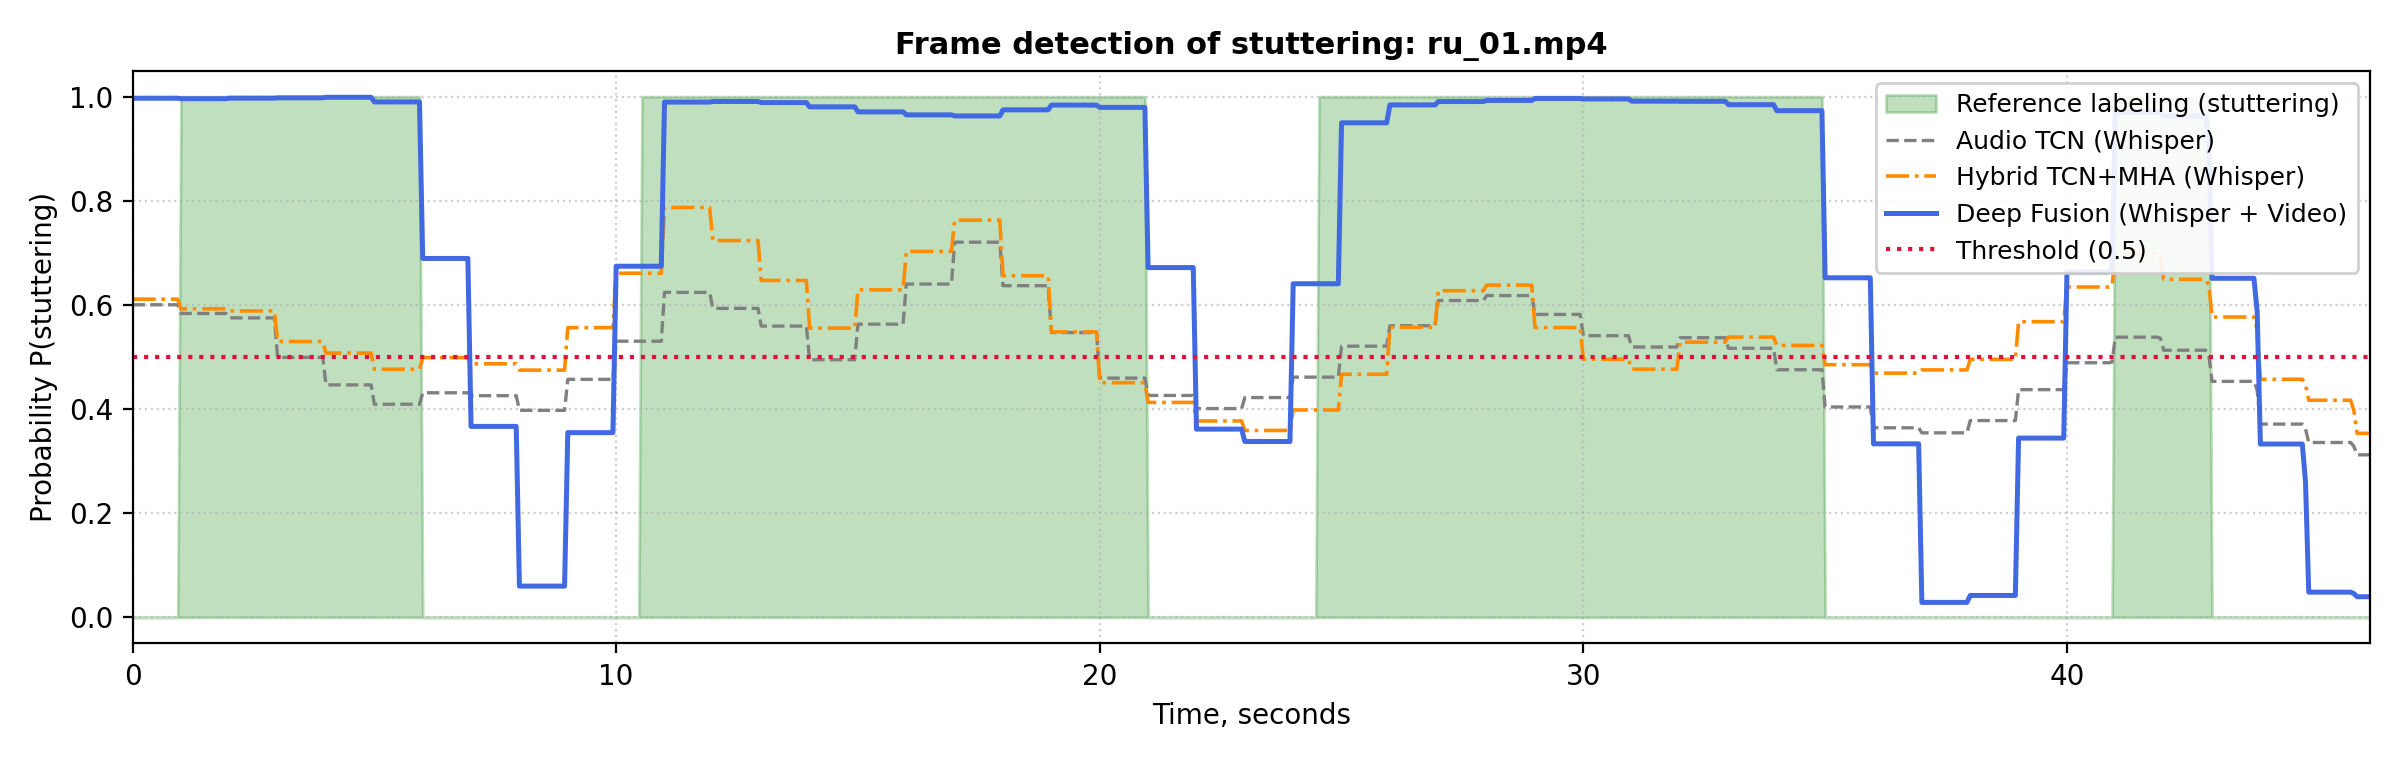
\includegraphics[width=0.92\textwidth]{../results/plots/timeline_ru_01.png}\vspace{0.15cm}
		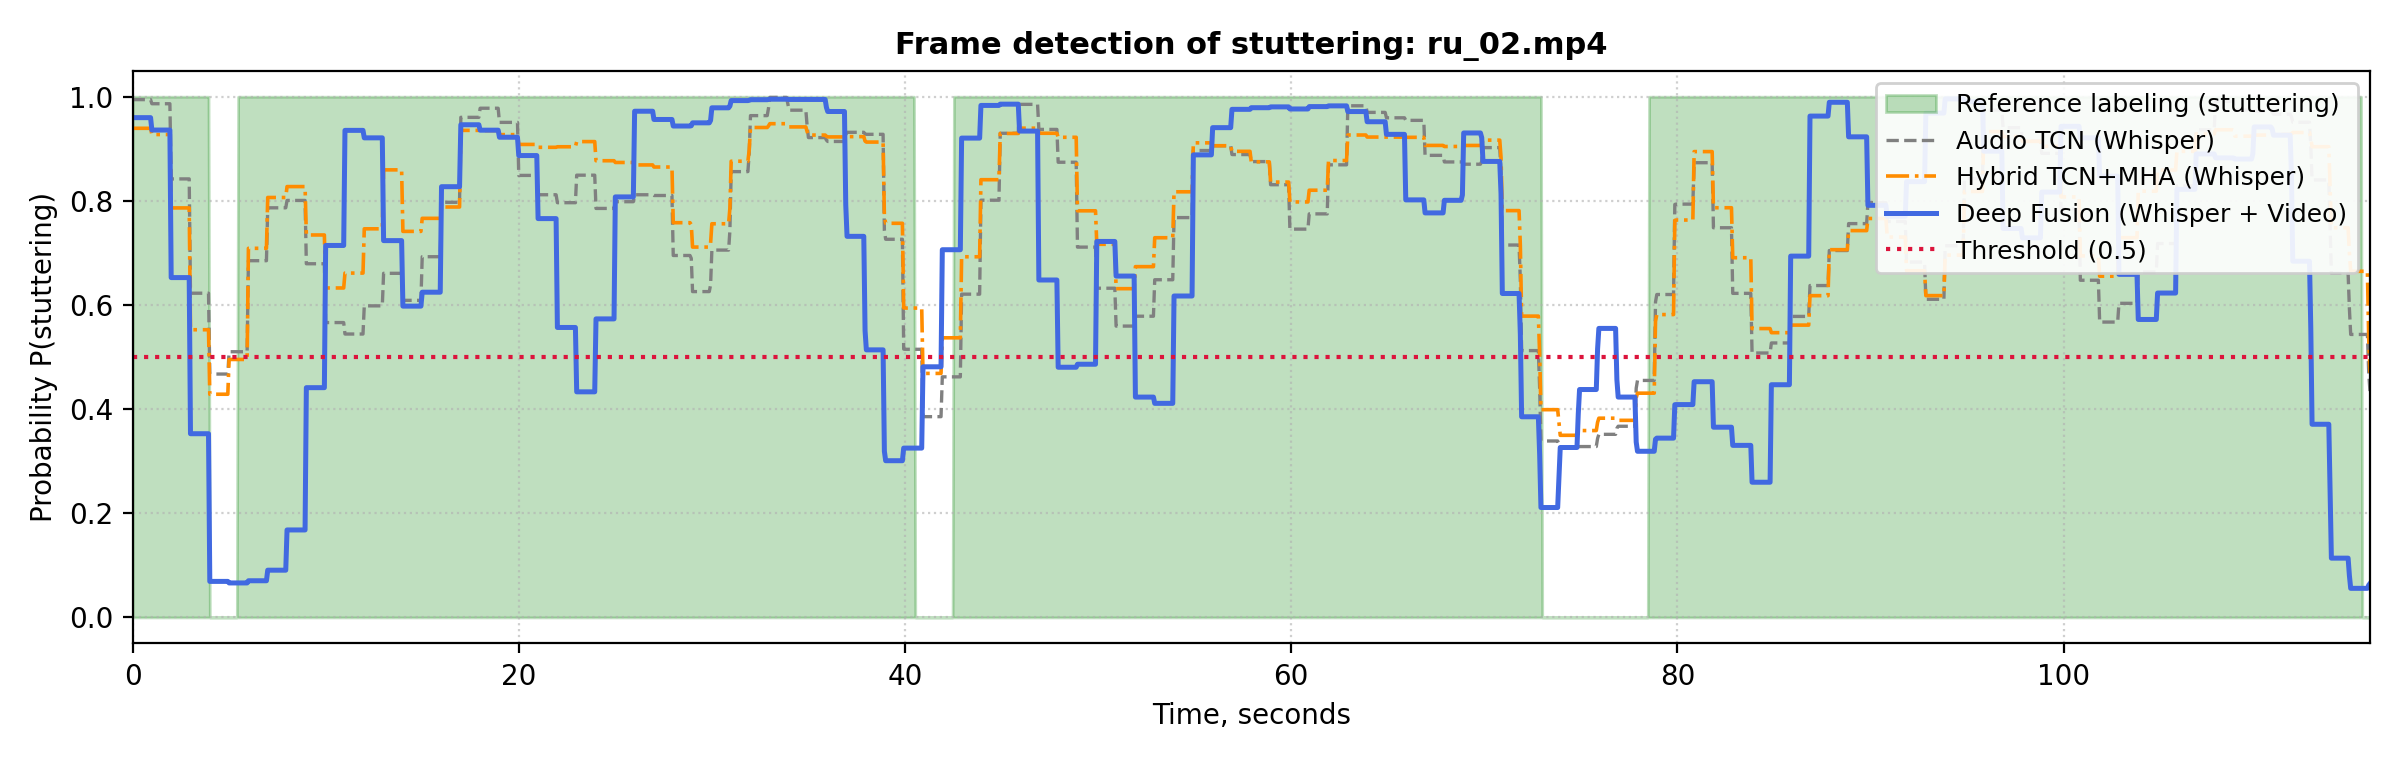
\includegraphics[width=0.92\textwidth]{../results/plots/timeline_ru_02.png}\vspace{0.15cm}
		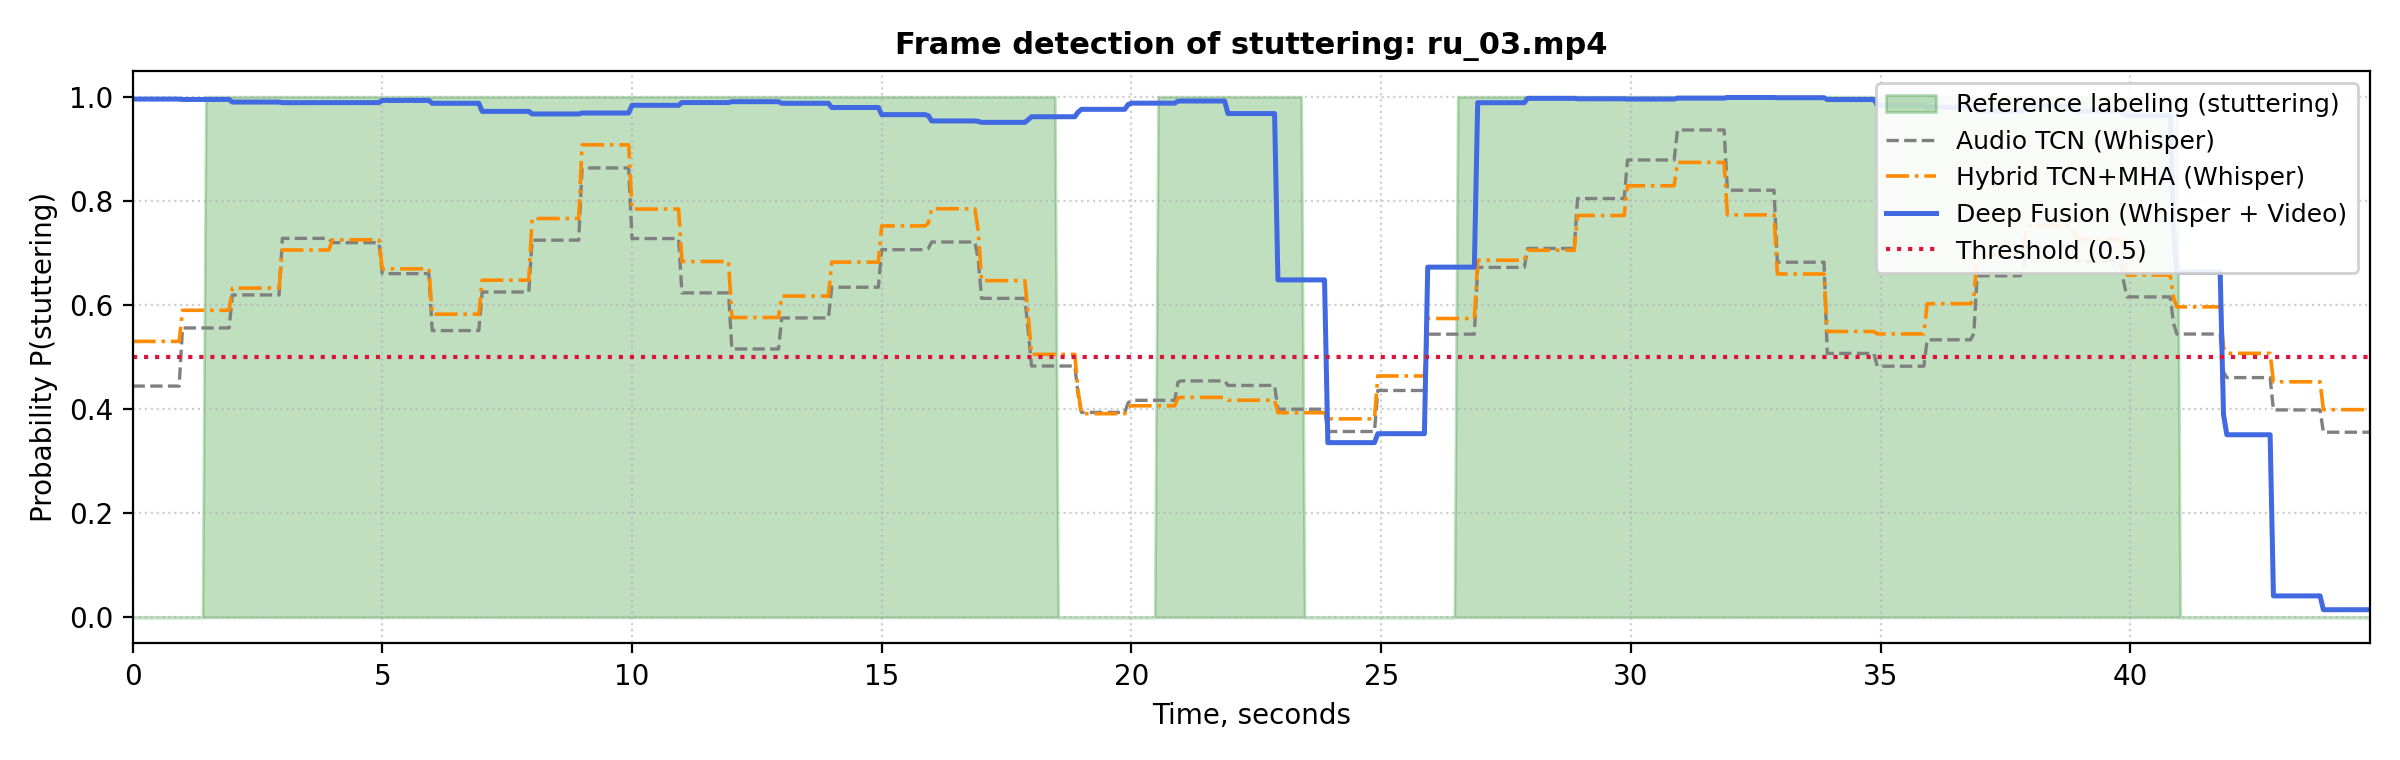
\includegraphics[width=0.92\textwidth]{../results/plots/timeline_ru_03.png}
		\caption{Покадровая сегментация эпизодов заикания скользящим окном на видеозаписях ru\_01.mp4, ru\_02.mp4 и ru\_03.mp4}
	\end{figure}
	
	\begin{figure}[h!]
		\centering
		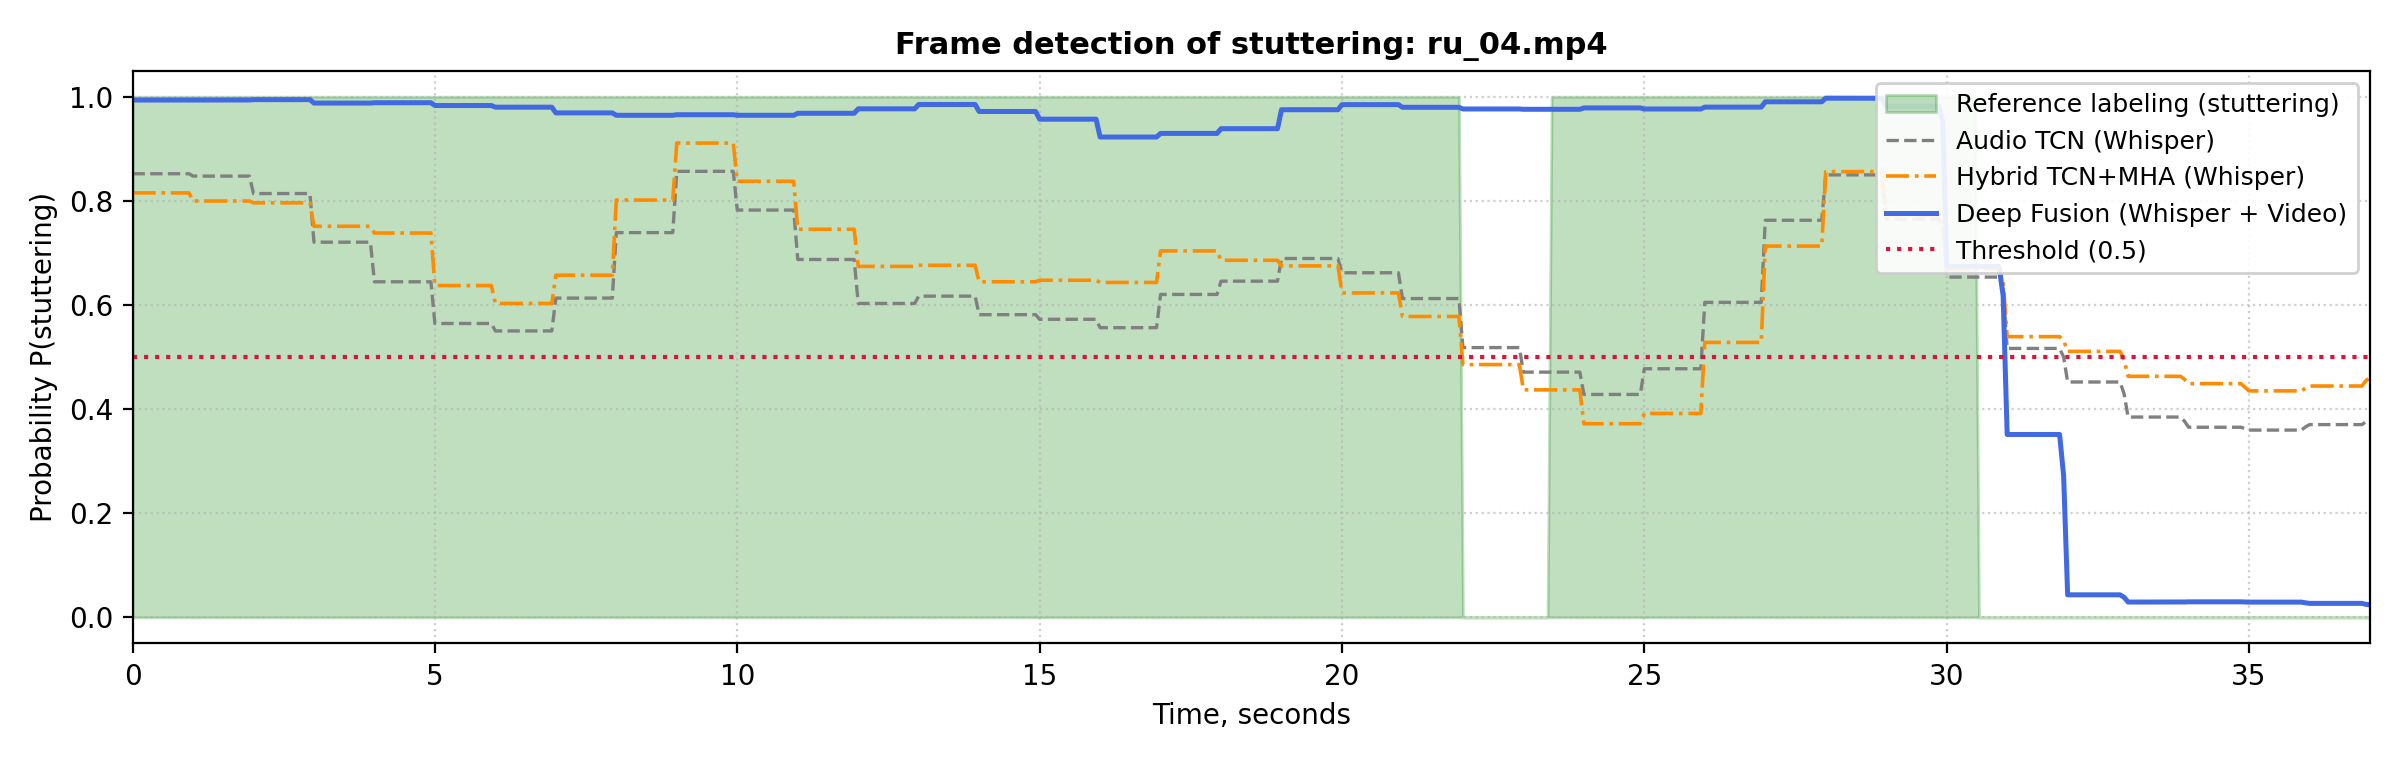
\includegraphics[width=0.92\textwidth]{../results/plots/timeline_ru_04.png}\vspace{0.15cm}
		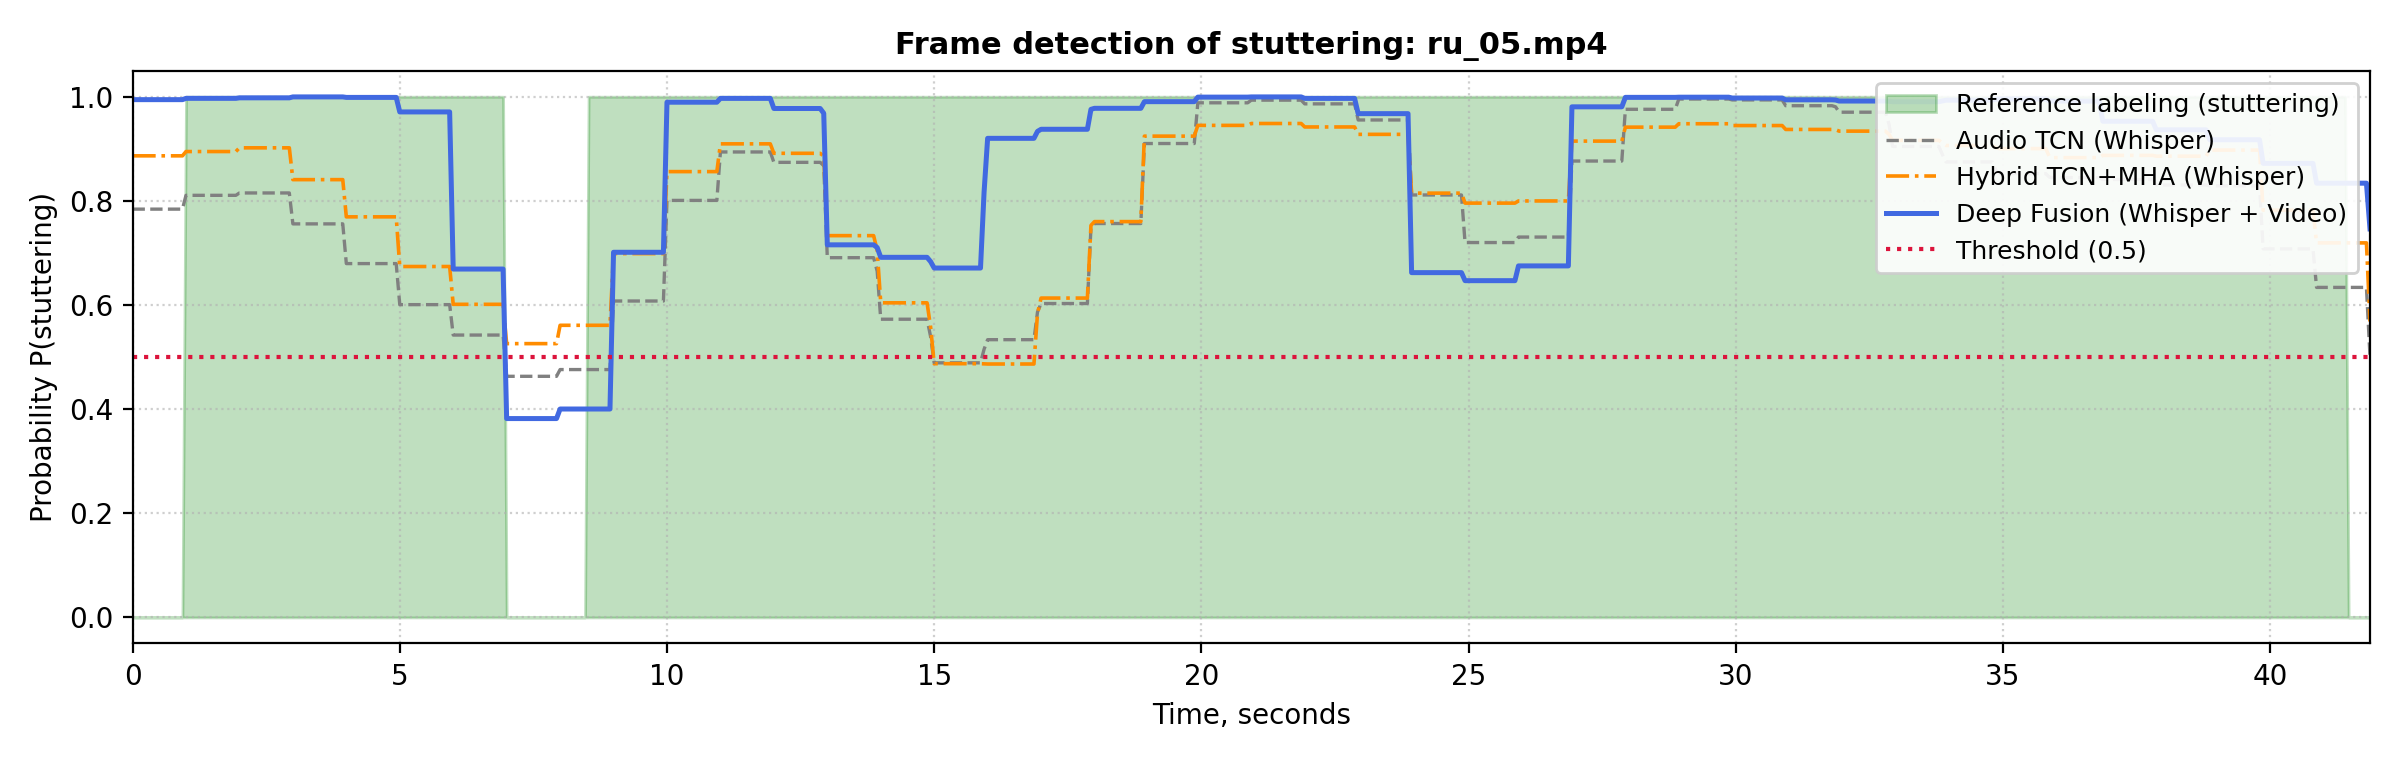
\includegraphics[width=0.92\textwidth]{../results/plots/timeline_ru_05.png}\vspace{0.15cm}
		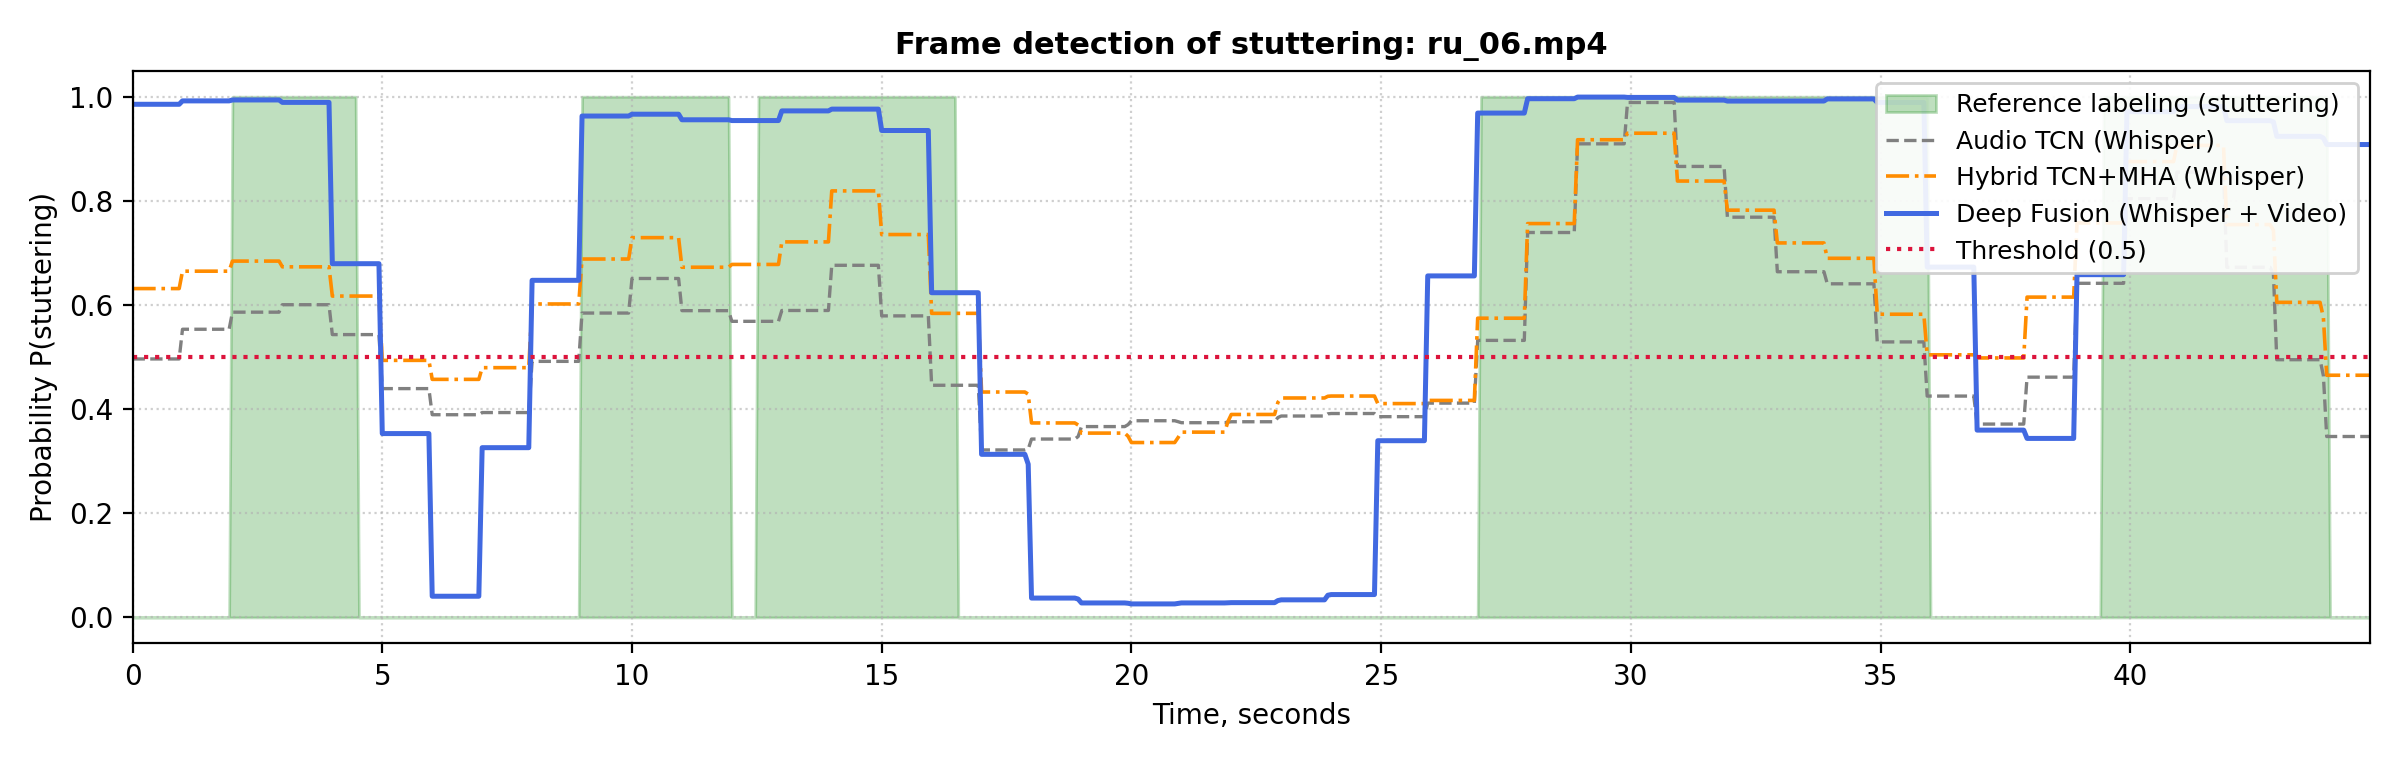
\includegraphics[width=0.92\textwidth]{../results/plots/timeline_ru_06.png}
		\caption{Покадровая сегментация эпизодов заикания скользящим окном на видеозаписях ru\_04.mp4, ru\_05.mp4 и ru\_06.mp4}
	\end{figure}
	
	Визуальный анализ полученных временных шкал выявляет три фундаментальных свойства разработанных алгоритмов:
	\begin{enumerate}
		\item высокая контрастность мультимодальной калибровки: на записях с чередованием патологических и чистых участков (ru\_01.mp4, ru\_06.mp4) одномодальные акустические модели формируют сглаженные траектории в диапазоне вероятностей $0.35\text{--}0.75$, тогда как сеть Deep Fusion демонстрирует близкую к прямоугольной передаточную характеристику, насыщаясь до $0.96\text{--}1.00$ внутри спазмов и опускаясь до $0.02\text{--}0.05$ на интервалах плавной речи (например, участок $17\text{--}25$ с на записи ru\_06.mp4);
		\item детекция акустически «немых» тонических блоков за счет видеоканала: на видеозаписи ru\_03.mp4 в интервале $20.5\text{--}23.5$ с наблюдается классический тонический блок (спазм речевого аппарата при полном отсутствии звукоизвлечения); обе чисто акустические модели (Audio TCN и Hybrid TCN + MHA) воспринимают этот участок как обычную интонационную паузу и опускают вероятность ниже порога ($P \approx 0.42$), допуская пропуск патологии, в то время как модель Deep Fusion за счет регистрации мышечного тремора и раскрытия рта удерживает вероятность на уровне $0.99$, безошибочно локализуя весь эпизод;
		\item эффект биомеханической инерции на сверхкоротких паузах: на записи ru\_04.mp4 в секундном промежутке между спазмами ($22.0\text{--}23.5$ с) акустические модели успевают кратковременно снизить оценку ниже $0.5$, тогда как мультимодальная сеть сохраняет высокий отклик, поскольку остаточное мышечное напряжение лица диктора не исчезает мгновенно в момент кратковременного прекращения фонации.
	\end{enumerate}
	
	\newpage
	\section*{Заключение}
	\addcontentsline{toc}{section}{Заключение}
	
	В результате выполнения производственной практики была спроектирована, математически обоснована и программно реализована полнофункциональная модульная система для автоматической мультимодальной детекции заиканий.
	
	Основные итоги и достижения проделанной работы заключаются в следующем:
	\begin{enumerate}
		\item сформирован и стандартизирован локальный корпус из 31 908 аудиозаписей SEP-28k \cite{sep28k}; проведен разведочный анализ, обосновавший применение фокальной функции потерь \cite{focalloss};
		\item разработана архитектура офлайн-экстракции пофреймовых признаков для трансформеров Wav2Vec2 \cite{wav2vec}, WavLM \cite{wavlm} и Whisper \cite{whisper} с внедрением механизма квантования кэша ОЗУ в формат float16, что снизило потребление памяти с 19.6 ГБ до 9.8 ГБ и обеспечило стабильное обучение на системе с 16 ГБ RAM и 6 ГБ VRAM;
		\item выявлен и аналитически доказан эффект коллапса мажоритарного класса при сохранении весов по F1-мере на несбалансированных данных; осуществлен переход на критерий максимизации ROC-AUC \cite{ivankin};
		\item доказано преимущество временных сверточных сетей \cite{tcn} над усреднением признаков: специфичность классификации на базе Wav2Vec2 выросла с $0.5172$ до $0.6795$;
		\item в ходе сравнительного тестирования установлено, что наилучшим качеством разделения обладает энкодер Whisper-Small \cite{whisper}: связка TCN + Whisper достигла рекордных показателей $\text{ROC-AUC} = 0.8488$, $\text{AP} = 0.9308$ и $\text{F1} = 0.8552$, а гибридная архитектура Hybrid TCN + MHA ($\text{ROC-AUC} = 0.8473$) позволила дополнительно повысить специфичность детекции на $+4.75$ п.п. (до $0.5971$) и точность до $0.8340$;
		\item сформирован и программно стандартизирован тестовый русскоязычный видеокорпус (6 видеозаписей, 4965 видеокадров и 16 565 аудиофреймов); разработаны и верифицированы модули автоматического аудита видимости лица: auto\_\allowbreak inspect\_\allowbreak videos.py, устранения артефактных заставок со сдвигом временной шкалы: trim\_\allowbreak intros.py, экстракции 42 биомеханических параметров лица на базе MediaPipe Face Mesh: extract\_\allowbreak face\_\allowbreak kinematics.py \cite{mediapipe} и блочного извлечения акустических признаков по трем архитектурам трансформеров: extract\_\allowbreak russian\_\allowbreak all\_\allowbreak audio.py;
		\item проведена полная кросс-языковая и мультимодальная валидация 12 конфигураций моделей при покадровой сегментации русской речи скользящим окном: evaluate\_\allowbreak crosslingual.py \cite{ivankin}; экспериментально доказано, что в режиме нулевого переноса (Zero-Shot) сверточная сеть Audio TCN на базе Whisper-Small достигает $\text{ROC-AUC} = 0.9576$, $\text{F1} = 0.9443$ и $\text{Specificity} = 0.8424$, а архитектура раннего глубокого слияния Deep Fusion позволяет повысить специфичность модели WavLM с $0.0422$ до $0.6088$ ($\text{ROC-AUC} = 0.9087$, $\text{F1} = 0.9298$) и обеспечить сбалансированную детекцию в связке с Whisper ($\text{ROC-AUC} = 0.8518$, $\text{F1} = 0.9062$, $\text{Specificity} = 0.6435$), существенно превосходя показатели лабораторных бейзлайнов \cite{ivankin}.
		\end{enumerate}
		
		Все поставленные задачи производственной практики выполнены в полном объеме. Разработанный программный комплекс верифицирован на реальных аудио- и видеоданных и готов к применению в системах клинического мониторинга и логопедической диагностики речевых нарушений \cite{ivankin}.
	
	\newpage
	\begin{thebibliography}{9}
		\addcontentsline{toc}{section}{Список литературы}
		\bibitem{ivankin}
		Ivankin E., Bazenkov N. Audio-Visual Stuttering Detection in Russian Video Recordings. Moscow Institute of Physics and Technology, 2026.
		\bibitem{sep28k}
		Lea C., Mitra V., Joshi A., Kajarekar S., Bigham J. P. SEP-28k: A Dataset for Stuttering Event Detection from Podcasts with People Who Stutter. ICASSP, 2021, pp. 6798--6802.
		\bibitem{wav2vec}
		Baevski A., Zhou H., Mohamed A., Auli M. wav2vec 2.0: A Framework for Self-Supervised Learning of Speech Representations. Advances in Neural Information Processing Systems (NeurIPS), 2020, vol. 33, pp. 12449--12460.
		\bibitem{wavlm}
		Chen S., Wang C., Chen Z. et al. WavLM: Large-Scale Self-Supervised Pre-Training for Full Stack Speech Processing. IEEE Journal of Selected Topics in Signal Processing, 2022, vol. 16, no. 6, pp. 1505--1518.
		\bibitem{whisper}
		Radford A., Kim J. W., Xu T. et al. Robust Speech Recognition via Large-Scale Weak Supervision. International Conference on Machine Learning (ICML), 2023, pp. 28492--28518.
		\bibitem{mediapipe}
		Lugaresi C., Tang J., Nash H. et al. MediaPipe: A Framework for Building Perception Pipelines. CVPR Workshop, 2019.
		\bibitem{tcn}
		Bai S., Kolter J. Z., Koltun V. An Empirical Evaluation of Generic Convolutional and Recurrent Networks for Sequence Modeling. arXiv preprint arXiv:1803.01271, 2018.
		\bibitem{focalloss}
		Lin T. Y., Goyal P., Girshick R., He K., Dollar P. Focal Loss for Dense Object Detection. IEEE International Conference on Computer Vision (ICCV), 2017, pp. 2980--2988.
	\end{thebibliography}
	
	\newpage
	\section*{Приложение А. Полные листинги программного кода}
	\addcontentsline{toc}{section}{Приложение А. Полные листинги программного кода}
	
	В данном приложении приведены регламент воспроизведения вычислительных экспериментов и полные исходные тексты всех разработанных программных модулей исследовательского конвейера (справочный модуль общих утилит и функций потерь utils.py приведен в разделе А.7).
	
	\subsection*{Регламент пошагового запуска программного конвейера}
	Для полного воспроизведения результатов исследования программные модули запускаются из корневой директории проекта в следующей технологической последовательности:
	
	Этап I. Базовый акустический конвейер на англоязычном корпусе SEP-28k:
	\begin{enumerate}
		\item загрузка, декодирование и стандартизация аудиокорпуса (раздел А.1):\\
		python scripts/sep28k\_data\_preparation.py
		\item разведочный анализ данных и распределения дисфлуенций (раздел А.2):\\
		python scripts/sep28k\_data\_analysis.py
		\item офлайн-экстракция агрегированных и пофреймовых признаков трансформеров (разделы А.3--А.6):\\
		python scripts/extract\_features.py\\
		python scripts/extract\_features\_seq.py\\
		python scripts/extract\_features\_wavlm.py\\
		python scripts/extract\_features\_whisper.py
		\item обучение базового перцептрона, сверточных сетей StutterTCN и гибридной сети с механизмом самовнимания (разделы А.8--А.10):\\
		python scripts/train\_mlp.py\\
		python scripts/train\_tcn.py --encoder\_name wav2vec2\\
		python scripts/train\_tcn.py --encoder\_name wavlm\\
		python scripts/train\_tcn.py --encoder\_name whisper\\
		python scripts/train\_hybrid\_tcn.py --encoder\_name whisper
		\item единая валидация акустических моделей и формирование Таблицы 1 (раздел А.11):\\
		python scripts/compare\_encoders.py
	\end{enumerate}
	
	Этап II. Подготовка русскоязычного видеокорпуса и мультимодальная валидация:
	\begin{enumerate}
		\setcounter{enumi}{5}
		\item автоматический аудит видеозаписей и первичная детекция заставок (раздел А.16):\\
		python scripts/auto\_inspect\_videos.py
		\item покадровая обрезка заставок через FFmpeg и синхронизация разметки (раздел А.17):\\
		python scripts/trim\_intros.py
		\item извлечение 42 параметров физической кинематики лица MediaPipe (раздел А.12):\\
		python scripts/extract\_face\_kinematics.py --video\_dir data/russian\_videos --output\_dir data/russian\_face\_kinematics --target\_fps 15
		\item блочная экстракция акустических признаков русской речи по трем трансформерам (раздел А.18):\\
		python scripts/extract\_russian\_all\_audio.py
		\item групповая кросс-валидация визуальной модели Face TCN и мультимодальных сетей раннего слияния DeepFusionTCN (разделы А.13--А.14):\\
		python scripts/train\_face\_tcn.py --features\_dir data/russian\_face\_kinematics --labels\_json data/russian\_labels.json --n\_folds 3\\
		python scripts/train\_deep\_fusion.py --encoder\_name wav2vec2 --audio\_dir data/russian\_seq\_wav2vec2 --video\_dir data/russian\_face\_kinematics --labels\_json data/russian\_labels.json --n\_folds 3\\
		python scripts/train\_deep\_fusion.py --encoder\_name wavlm --audio\_dir data/russian\_seq\_wavlm --video\_dir data/russian\_face\_kinematics --labels\_json data/russian\_labels.json --n\_folds 3\\
		python scripts/train\_deep\_fusion.py --encoder\_name whisper --audio\_dir data/russian\_seq\_whisper --video\_dir data/russian\_face\_kinematics --labels\_json data/russian\_labels.json --n\_folds 3
		\item финальное покадровое тестирование скользящим окном, генерация Таблицы 3 и графиков временных шкал (раздел А.15):\\
		python scripts/evaluate\_crosslingual.py
	\end{enumerate}
	
	\subsection*{А.1. Скрипт загрузки и стандартизации датасета (sep28k\_data\_preparation.py)}
	\lstinputlisting[language=Python]{../scripts/sep28k_data_preparation.py}
	
	\subsection*{А.2. Скрипт разведочного анализа данных (sep28k\_data\_analysis.py)}
	\lstinputlisting[language=Python]{../scripts/sep28k_data_analysis.py}
	
	\subsection*{А.3. Извлечение агрегированных признаков (extract\_features.py)}
	\lstinputlisting[language=Python]{../scripts/extract_features.py}
	
	\subsection*{А.4. Пофреймовая экстракция Wav2Vec2 (extract\_features\_seq.py)}
	\lstinputlisting[language=Python]{../scripts/extract_features_seq.py}
	
	\subsection*{А.5. Пофреймовая экстракция WavLM (extract\_features\_wavlm.py)}
	\lstinputlisting[language=Python]{../scripts/extract_features_wavlm.py}
	
	\subsection*{А.6. Пофреймовая экстракция Whisper (extract\_features\_whisper.py)}
	\lstinputlisting[language=Python]{../scripts/extract_features_whisper.py}
	
	\subsection*{А.7. Общие утилиты, функции потерь и оптимизация ОЗУ (utils.py)}
	\lstinputlisting[language=Python]{../scripts/utils.py}
	
	\subsection*{А.8. Обучение базового классификатора MLP (train\_mlp.py)}
	\lstinputlisting[language=Python]{../scripts/train_mlp.py}
	
	\subsection*{А.9. Архитектура и обучение временной сверточной сети (train\_tcn.py)}
	\lstinputlisting[language=Python]{../scripts/train_tcn.py}
	
	\subsection*{А.10. Гибридная архитектура TCN + Multi-Head Attention (train\_hybrid\_tcn.py)}
	\lstinputlisting[language=Python]{../scripts/train_hybrid_tcn.py}
	
	\subsection*{А.11. Сравнение акустических энкодеров (compare\_encoders.py)}
	\lstinputlisting[language=Python]{../scripts/compare_encoders.py}
	
	\subsection*{А.12. Извлечение физической кинематики лица (extract\_face\_kinematics.py)}
	\lstinputlisting[language=Python]{../scripts/extract_face_kinematics.py}
	
	\subsection*{А.13. Обучение визуального классификатора (train\_face\_tcn.py)}
	\lstinputlisting[language=Python]{../scripts/train_face_tcn.py}
	
	\subsection*{А.14. Архитектура и обучение мультимодальной сети (train\_deep\_fusion.py)}
	\lstinputlisting[language=Python]{../scripts/train_deep_fusion.py}
	
	\subsection*{А.15. Скрипт кросс-языковой валидации и визуализации (evaluate\_crosslingual.py)}
	\lstinputlisting[language=Python]{../scripts/evaluate_crosslingual.py}
	
	\subsection*{А.16. Модуль инспекции видео и предварительной детекции (auto\_inspect\_videos.py)}
	\lstinputlisting[language=Python]{../scripts/auto_inspect_videos.py}
	
	\subsection*{А.17. Автоматическая обрезка заставок и синхронизация разметки (trim\_intros.py)}
	\lstinputlisting[language=Python]{../scripts/trim_intros.py}
	
	\subsection*{А.18. Мультиэнкодерная блочная экстракция аудиопризнаков (extract\_russian\_all\_audio.py)}
	\lstinputlisting[language=Python]{../scripts/extract_russian_all_audio.py}
\end{document}